\ifdefined\maindoc\else
% typesetting this chapter as a standalone document
\def\doctitle{Simulation Control}
% starting definitions for both the main document and stand-alone chapters
\documentclass{book}

\def\mech{artisynth.core.mechmodels}
\def\mgeo{maspack.geometry}

% Add search paths for input files
\makeatletter
\def\input@path{{../}{../../}{../texinputs/}}
\makeatother

\usepackage{amsmath}
\usepackage{framed}
%%
%% Default settings for artisynth
%%
\NeedsTeXFormat{LaTeX2e}
%%\ProvidesPackage{artisynthDoc}[2012/04/05]

\usepackage[T1]{fontenc}
\usepackage[latin1]{inputenc}
\usepackage{listings}
\usepackage{makeidx}
\usepackage{latexml}
\usepackage{graphicx}
\usepackage{framed}
\usepackage{booktabs}
\usepackage{color}

\newcommand{\pubdate}{\today}
\newcommand{\setpubdate}[1]{\renewcommand{\pubdate}{#1}}
\newcommand{\code}[1]{{\tt #1}}

\iflatexml
\usepackage{hyperref}
\setlength\parindent{0pt} 
\else
%% then we are making a PDF, so include things that LaTeXML can't handle: 
%% docbook style, \RaggedRight
\usepackage{ifxetex}
\usepackage{xstring}
\usepackage{pslatex} % fixes fonts; in particular sets a better-fitting \tt font

\usepackage[most]{tcolorbox}
\definecolor{shadecolor}{rgb}{0.95,0.95,0.95}
\tcbset{
    frame code={}
    center title,
    left=0pt,
    right=0pt,
    top=0pt,
    bottom=0pt,
    colback=shadecolor,
    colframe=white,
    width=\dimexpr\textwidth\relax,
    enlarge left by=0mm,
    boxsep=0pt,
    arc=0pt,outer arc=0pt,
}%

\usepackage[A4]{artisynth_papersize}
%\usepackage[letter]{artisynth_papersize}
\usepackage[hyperlink]{asciidoc-dblatex} 

%\usepackage{verbatim}
\usepackage{ragged2e}
\setlength{\RaggedRightRightskip}{0pt plus 4em}
\RaggedRight
\renewcommand{\DBKpubdate}{\pubdate}
\renewcommand{\DBKreleaseinfo}{}
\fi

% set hypertext links to be dark blue:
\definecolor{darkblue}{rgb}{0,0,0.8}
\definecolor{sidebar}{rgb}{0.5,0.5,0.7}
\hypersetup{colorlinks=true,urlcolor=darkblue,linkcolor=darkblue,breaklinks=true}

%%%%%%%%%%%%%%%%%%%%%%%%%%%%%%%%%%%%%%%%%%%%%%%%%%%%%%%%%%%%%%%%%%%%%%%%%%%%%
%
% Define macros for handling javadoc class and method references
%
%%%%%%%%%%%%%%%%%%%%%%%%%%%%%%%%%%%%%%%%%%%%%%%%%%%%%%%%%%%%%%%%%%%%%%%%%%%%%
\makeatletter

% macro to enable line break if inside a PDF file
\def\pdfbreak{\iflatexml\else\\\fi}

% code inspired by http://stackoverflow.com/questions/2457780/latex-apply-an-operation-to-every-character-in-a-string
\def\removeargs #1{\doremoveargs#1$\wholeString\unskip}
\def\doremoveargs#1#2\wholeString{\if#1$%
\else\if#1({()}\else{#1}\taketherest#2\fi\fi}
\def\taketherest#1\fi
{\fi \doremoveargs#1\wholeString}

% Note: still doesn't work properly when called on macro output ...
% i.e., \dottoslash{\concatnames{model}{base}{foo}} fails 
\def\dottoslash #1{\dodottoslash#1$\wholeString\unskip}
\def\dodottoslash#1#2\wholeString{\if#1$%
\else\if#1.{/}\else{#1}\fi\dottaketherest#2\fi}
\def\dottaketherest#1\fi{\fi \dodottoslash#1\wholeString}

\def\hashtodot #1{\dohashtodot#1$\wholeString\unskip}
\def\dohashtodot#1#2\wholeString{\if#1$X%
\else\if#1\#{.}\else{#1}\fi\hashtaketherest#2\fi}
\def\hashtaketherest#1\fi{\fi \dohashtodot#1\wholeString}

%\dollartodot{#1} does the same thing as \StrSubstitute[0]{#1}{\$}{.}
% from the packahe xstring. We define \dollartodot instead because
% LaTeXML does not implement xstring.
%
% Note that for the substituion to work, we need \ifx instead of \if,
% since otherwise escaped characters won't work properly:
% if #1 = \$, then \if#1* seems to compare '\' and '$' (and output '*'),
% rather than comparing '$' to '*'
\def\dollartodot #1{\dodollartodot#1*\wholeString\unskip}
\def\dodollartodot#1#2\wholeString{\ifx#1*%
\else \ifx#1\${.}\else{#1}\fi\dollartaketherest#2\fi}
\def\dollartaketherest#1\fi{\fi \dodollartodot#1\wholeString}

% concatenates up to three class/method names together, adding '.' characters
% between them. The first and/or second argument may be empty, in which case
% the '.' is omitted. To check to see if these arguments are empty, we
% use a contruction '\if#1@@', which will return true iff #1 is empty
% (on the assumption that #1 will not contain a '@' character).
\def\concatnames
#1#2#3{\if#1@@\if#2@@#3\else #2.#3\fi\else\if#2@@#1.#3\else#1.#2.#3\fi\fi}

\newcommand{\javabase}{}
\newcommand{\setjavabase}[1]{\renewcommand{\javabase}{#1}}

\def\artisynthDocBase{@ARTISYNTHDOCBASE}

\iflatexml
\def\ifempty#1{\def\temp{#1}\ifx\temp\empty}%
\newcommand{\artisynthManual}[3][]{%
   \ifempty{#1}
      \href{@ARTISYNTHDOCBASE/#2/#2.html}{#3}%
    \else
      \href{@ARTISYNTHDOCBASE/#1/#2.html}{#3}%
    \fi
}
\else
\newcommand{\artisynthManual}[3][]{%
\href{https://www.artisynth.org/@ARTISYNTHDOCBASE/#2.pdf}{#3}}
\fi

%\href{@ARTISYNTHDOCBASE/#2/#2.html}{#3}}



\newcommand{\javaclassx}[2][]{%
% Includes code to prevent an extra '.' at the front if #1 is empty. It
% works like this: if '#1' is empty, then '#1.' expands to '.', and so 
% '\if#1..' will return true, in which case we just output '#2'.
\href{@JDOCBEGIN/\concatnames{\javabase}{#1}{#2}@JDOCEND}{#2}}
\newcommand{\javaclass}[2][]{%
\href{@JDOCBEGIN/\concatnames{}{#1}{#2}@JDOCEND}{\dollartodot{#2}}}
\newcommand{\javaclassAlt}[2]{%
\href{@JDOCBEGIN/\concatnames{}{}{#1}@JDOCEND}{#2}}

\newcommand{\javamethodArgsx}[2][]{%
\href{@JDOCBEGIN/\concatnames{\javabase}{#1}{#2}@JDOCEND}{#2}}
\newcommand{\javamethodArgs}[2][]{%
\href{@JDOCBEGIN/\concatnames{}{#1}{#2}@JDOCEND}{#2}}
\newcommand{\javamethodAlt}[2]{%
\href{@JDOCBEGIN/\concatnames{}{}{#1}@JDOCEND}{#2}}
\newcommand{\javamethodAltx}[2]{%
\href{@JDOCBEGIN/\concatnames{\javabase}{}{#1}@JDOCEND}{#2}}

\newcommand{\javamethodNoArgsx}[2][]{%
\href{@JDOCBEGIN/\concatnames{\javabase}{#1}{#2}@JDOCEND}{\removeargs{#2}}}
\newcommand{\javamethodNoArgs}[2][]{%
\href{@JDOCBEGIN/\concatnames{}{#1}{#2}@JDOCEND}{\removeargs{#2}}}

\newcommand{\javamethod}{\@ifstar\javamethodNoArgs\javamethodArgs}
\newcommand{\javamethodx}{\@ifstar\javamethodNoArgsx\javamethodArgsx}

%%%%%%%%%%%%%%%%%%%%%%%%%%%%%%%%%%%%%%%%%%%%%%%%%%%%%%%%%%%%%%%%%%%%%%%%%%%%%
%
% Define macros for sidebars
%
%%%%%%%%%%%%%%%%%%%%%%%%%%%%%%%%%%%%%%%%%%%%%%%%%%%%%%%%%%%%%%%%%%%%%%%%%%%%%

\iflatexml
\newenvironment{sideblock}{\begin{quote}}{\end{quote}}
\else
\usepackage[strict]{changepage}
\definecolor{sidebarshade}{rgb}{1.0,0.97,0.8}
\newenvironment{sideblock}{%
    \def\FrameCommand{%
    \hspace{1pt}%
    {\color{sidebar}\vrule width 2pt}%
    %{\vrule width 2pt}%
    {\color{sidebarshade}\vrule width 4pt}%
    \colorbox{sidebarshade}%
  }%
  \MakeFramed{\advance\hsize-\width\FrameRestore}%
  \noindent\hspace{-4.55pt}% disable indenting first paragraph
  \begin{adjustwidth}{}{7pt}%
  %\vspace{2pt}\vspace{2pt}%
}
{%
  \vspace{2pt}\end{adjustwidth}\endMakeFramed%
}
\fi

\iflatexml
\newenvironment{shadedregion}{%
  \definecolor{shadecolor}{rgb}{0.96,0.96,0.98}%
  \begin{shaded*}%
% Put text inside a quote to create a surrounding blockquote that
% will properly accept the color and padding attributes
  \begin{quote}%
}
{%
  \end{quote}%
  \end{shaded*}%
}
\else
\newenvironment{shadedregion}{%
  \definecolor{shadecolor}{rgb}{0.96,0.96,0.98}%
  \begin{shaded*}%
}
{%
  \end{shaded*}%
}
\fi

% Wanted to create a 'listing' environment because lstlisting is
% tedious to type and because under latexml it may need
% some massaging to get it to work properly. But hard to do
% because of the verbatim nature of listing
%\iflatexml
%\newenvironment{listing}{\begin{lstlisting}}{\end{lstlisting}}%
%\else
%\newenvironment{listing}{\begin{lstlisting}}{\end{lstlisting}}%
%\fi

\iflatexml\else
% fancyhdr was complaining that it wanted a 36pt header height ...
\setlength{\headheight}{36pt}
\fi

% macro for backslash character
\newcommand\BKS{\textbackslash}

% macro for double hyphen (to prevent conversion of -- into -)
\newcommand\DHY{-{}-}

% Convenience stuff
\newcommand{\ifLaTeXMLelse}[2]{%
  \iflatexml %
  #1 %
  \else %
  #2 %
  \fi %
}

\newcommand{\ifLaTeXML}[1]{ %
  \iflatexml %
  #1 %
  \fi %
}

% new methodtable environment for documenting methods

% base width of the method table
\newlength{\methodtablewidth}
\iflatexml
\setlength{\methodtablewidth}{1.4\textwidth}
\else
\setlength{\methodtablewidth}{0.94\textwidth}
\fi
% horizontal space added at end of call to \methodentry
\newlength{\methodskip}
\setlength{\methodskip}{0pt}
% lengths set inside methodtable environment:
\newlength{\methodsiglength} % length of the method signature
\newlength{\methodcomlength} % length of the method comment
\setlength{\methodsiglength}{0.5\methodtablewidth}
\setlength{\methodcomlength}{0.5\methodtablewidth}

% command to add a method to a method table:
% arg #1: package and signature for finding URL
% arg #2: anchor text
% arg #3: comment describing the method
\newcommand{\methodentry}[3]{%
\javamethodAlt{#1}{\parbox[t]{\methodsiglength}{#2}}&
{\parbox[t]{\methodcomlength}{#3}}\\%
\noalign{\vspace{\methodskip}}}

% methodtable environment takes two arguments, both scale factors for
% methodtablewidth:
% arg #1: width of the method signature column
% arg #2: width of the method comment column
\newenvironment{methodtable}[3][0pt]{%
\begingroup
\setlength{\topskip}{0pt}
\setlength{\methodskip}{#1}
\setlength{\methodsiglength}{#2\methodtablewidth}%
\setlength{\methodcomlength}{#3\methodtablewidth}%
\iflatexml
\begin{snugshade}
\else
\begin{tcolorbox}
\fi
\renewcommand{\arraystretch}{1}
\begin{tabular}{ll}}{%
\end{tabular}
\renewcommand{\arraystretch}{1}
\iflatexml
\end{snugshade}
\else
\end{tcolorbox}
\fi
\endgroup}

% commands for added top, mid and bottom lines in the table.
% uses booktabs for PDF, regular hline for HTML
\newcommand{\topline}{\iflatexml\hline\else\toprule\fi}
\newcommand{\midline}{\iflatexml\hline\else\midrule\fi}
\newcommand{\botline}{\iflatexml\hline\else\bottomrule\fi}
\newcommand{\blankline}{%
\multicolumn{2}{l}{\iflatexml{@SPACE}\else\phantom{M}\fi}\\}%
% add vertical space within a two colum method environment
\newcommand{\methodspace}[1]{%
\iflatexml
\multicolumn{2}{l}{@VERTSPACE[#1]}\\
\else
\noalign{\vspace{#1}}%
\fi}%
% break a line and add an indentation of 1em
\newcommand{\brh}{\\\phantom{M}}

\makeatother

\def\matl{\left(\begin{matrix}}
\def\matr{\end{matrix}\right)}

\def\Bthe{\boldsymbol\theta}
\def\Btau{\boldsymbol\tau}
\def\Bom{\boldsymbol\omega}
\def\Bdel{\boldsymbol\delta}
\def\Blam{\boldsymbol\lambda}
\def\Bphi{\boldsymbol\phi}
\def\Bxi{\boldsymbol\xi}
\def\Bgam{\boldsymbol\gamma}
\def\Bsig{\boldsymbol\sigma}
\def\Bnu{\boldsymbol\nu}
\def\Bmu{\boldsymbol\mu}

\def\A{{\bf A}}
\def\B{{\bf B}}
\def\C{{\bf C}}
\def\D{{\bf D}}
\def\F{{\bf F}}
\def\G{{\bf G}}
\def\H{{\bf H}}
\def\I{{\bf I}}
\def\J{{\bf J}}
\def\K{{\bf K}}
\def\Jc{{\bf J}_c}
\def\L{{\bf L}}
\def\M{{\bf M}}
\def\N{{\bf N}}
\def\O{{\bf O}}
\def\P{{\bf P}}
\def\Q{{\bf Q}}
\def\R{{\bf R}}
\def\T{{\bf T}}
\def\U{{\bf U}}
\def\W{{\bf W}}
\def\X{{\bf X}}
\def\Minv{{\bf M}^{-1}}

\def\a{{\bf a}}
\def\b{{\bf b}}
\def\c{{\bf c}}
\def\d{{\bf d}}
\def\e{{\bf e}}
\def\f{{\bf f}}
\def\g{{\bf g}}
\def\k{{\bf k}}
\def\l{{\bf l}}
\def\m{{\bf m}}
\def\n{{\bf n}}
\def\p{{\bf p}}
\def\q{{\bf q}}
\def\r{{\bf r}}
\def\u{{\bf u}}
\def\v{{\bf v}}
\def\w{{\bf w}}
\def\x{{\bf x}}
\def\y{{\bf y}}
\def\z{{\bf z}}

\def\ma{{\bf m}_\alpha}
\def\mb{{\bf m}_\beta}
\def\va{{\bf v}_\alpha}
\def\vb{{\bf v}_\beta}
\def\vp{{\bf v}_\rho}
\def\vk{{\bf v}_k}
\def\ua{{\bf u}_\alpha}
\def\ub{{\bf u}_\beta}
\def\uk{{\bf u}_k}
\def\uj{{\bf u}_j}
\def\mar{{\bf m}_{\alpha r}}
\def\mbr{{\bf m}_{\beta r}}

\def\Maa{{\bf M}_{\alpha\alpha}}
\def\Mab{{\bf M}_{\alpha\beta}}
\def\Mba{{\bf M}_{\beta\alpha}}
\def\Mbb{{\bf M}_{\beta\beta}}
\def\hatMaa{\hat{\bf M}_{\alpha\alpha}}
\def\hatMab{\hat{\bf M}_{\alpha\beta}}
\def\hatMba{\hat{\bf M}_{\beta\alpha}}
\def\hatMbb{\hat{\bf M}_{\beta\beta}}
\def\Mbp{{\bf M}_{\beta\rho}}
\def\Map{{\bf M}_{\alpha\rho}}
\def\Mpa{{\bf M}_{\rho\alpha}}
\def\Mpb{{\bf M}_{\rho\beta}}
\def\Mpp{{\bf M}_{\rho\rho}}
\def\Mbk{{\bf M}_{\beta k}}
\def\Mak{{\bf M}_{\alpha k}}
\def\Mka{{\bf M}_{k\alpha}}
\def\Mkb{{\bf M}_{k\beta}}
\def\Mkk{{\bf M}_{kk}}

\def\Ga{{\bf G}_{\alpha}}
\def\Gp{{\bf G}_{\rho}}
\def\Gaa{{\bf G}_{\alpha\alpha}}
\def\Gab{{\bf G}_{\alpha\beta}}
\def\Gba{{\bf G}_{\beta\alpha}}
\def\Gbb{{\bf G}_{\beta\beta}}
\def\Gap{{\bf G}_{\alpha\rho}}
\def\Gpa{{\bf G}_{\rho\alpha}}
\def\Gbp{{\bf G}_{\beta\rho}}
\def\Gak{{\bf G}_{\alpha k}}
\def\Gka{{\bf G}_{k\alpha}}
\def\Gja{{\bf G}_{j\alpha}}
\def\Gkb{{\bf G}_{k\beta}}
\def\Gbk{{\bf G}_{\beta k}}

\def\lama{\Blam_{\alpha}}
\def\lamb{\Blam_{\beta}}
\def\lamp{\Blam_{\rho}}
\def\lamk{\Blam_{k}}
\def\lams{\Blam_{\sigma}}

\def\ba{{\bf b}_{\alpha}}
\def\bb{{\bf b}_{\beta}}
\def\fp{{\bf f}_{\rho}}
\def\fa{{\bf f}_{\alpha}}
\def\qa{{\bf q}_{\alpha}}
\def\qb{{\bf q}_{\beta}}
\def\za{{\bf z}_{\alpha}}
\def\zb{{\bf z}_{\beta}}
\def\wa{{\bf w}_{\alpha}}
\def\wb{{\bf w}_{\beta}}

\def\Na{\bar{\bf N}_{\alpha}}
\def\Nb{\bar{\bf N}_{\beta}}

\def\Up{{\bf U}_p}
\def\Un{{\bf U}_n}

\def\dFdl{\frac{\partial F}{\partial l}}
\def\dFddl{\frac{\partial F}{\partial \dot l}}

\def\Sr{s_\theta}
\def\Cr{c_\theta}
\def\Sp{s_\phi}
\def\Cp{c_\phi}
\def\Sy{s_\psi}
\def\Cy{c_\psi}
\def\Sa{s_{\alpha}}
\def\Ca{c_{\alpha}}
\def\Vp{v_{\phi}}


\iflatexml
\else
\usepackage{biblatex}
\addbibresource{references.bib}
\fi

\setcounter{tocdepth}{5}
\setcounter{secnumdepth}{3}

\title{\doctitle}
\ifdefined\maindoc
\author{John Lloyd and Antonio S\'anchez}
\setpubdate{Last update: March, 2022}

\iflatexml
\date{}
\fi
\fi

% graphics paths
\graphicspath{{./}{images/}}

% Listings settings
\definecolor{myblue}{rgb}{0,0,0.6}
\definecolor{mygreen}{rgb}{0,0.6,0}
\definecolor{mygray}{rgb}{0.5,0.5,0.5}
\definecolor{mylightgray}{rgb}{0.95,0.95,0.95}
\definecolor{mymauve}{rgb}{0.58,0,0.82}
\definecolor{myblack}{rgb}{0,0,0}
\lstset{
   language=Java,                   % text highlighting for Java
   breakatwhitespace=false,         % automatic breaks only at whitespace
   breaklines=true,                 % automatic line breaking
   commentstyle=\color{mygreen},    % comment style
   keepspaces=true,                 % keeps spaces in text
   keywordstyle=\color{myblue},     % keyword style
   numbers=none,                    % line-numbers; values: (none, left, right)
   numbersep=5pt,                   % how far the line-numbers are from code
   numberstyle=\tiny\color{mygray}, % line-numbers style
   showspaces=false,                % show spaces everywhere
   showstringspaces=false,          % underline spaces within strings
   showtabs=false,                  % show tabs
   stepnumber=1,                    % the step between two line-numbers
   stringstyle=\color{mymauve},     % string literal style
   tabsize=3,                       % sets default tabsize to 3 spaces
   backgroundcolor=\color{mylightgray}, % background color
   frame=single, 					% adds a frame around the code
   rulesepcolor=\color{mygray},
   rulecolor=\color{myblack},
   framerule=0pt,
   xleftmargin=2.2ex,               % numbers inside box
   framexleftmargin=2.2ex,			% indentation of frame
}

\begin{document}

\frontmatter

%\layout
\maketitle

\iflatexml{\large\pubdate}\fi

\tableofcontents

\mainmatter
\fi

\chapter{Simulation Control}
\label{SimulationControl:sec}

This section describes different devices which an application may use
to control the simulation. These include {\it control panels} to allow
for the interactive adjustment of properties, as well as {\it agents}
which are applied every time step. Agents include {\it controllers}
and {\it input probes} to supply and modify input parameters at the
beginning of each time step, and {\it monitors} and {\it output
probes} to observe and record simulation results at the end of each
time step.

\section{Control Panels}
\label{ControlPanels:sec}

A {\it control panel} is an editing panel that allows for the
interactive adjustment of component properties.

It is always possible to adjust component properties through the GUI
by selecting one or more components and then choosing {\sf Edit
properties ...} in the right-click context menu. However, it may be
tedious to repeatedly select the required components, and the
resulting panels present the user with {\it all} properties common to
the selection.  A control panel allows an application to provide a
customized editing panel for selected properties.

\begin{sideblock}
If an application wishes to adjust an attribute that is not exported
as a property of some ArtiSynth component, it is often possible to
create a {\it custom property} for the attribute in question.
Custom properties are described in Section \ref{CustomProperties:sec}.
\end{sideblock}

\subsection{General principles}
\label{ControlPanelGeneral:sec}

Control panels are implemented by the
\javaclass[artisynth.core.gui]{ControlPanel} model component.  They
can be set up within a model's {\tt build()} method by creating an
instance of {\tt ControlPanel}, populating it with widgets for editing
the desired properties, and then adding it to the root model using the
latter's
\javamethod*[artisynth.core.workspace.RootModel]{addControlPanel()}
method. A typical code sequence looks like this:
%
\begin{lstlisting}[]
 ControlPanel panel = new ControlPanel ("controls");
 ... add widgets ... 
 addControlPanel (panel);
\end{lstlisting}
%

There are various {\tt addWidget()} methods available for adding
widgets and components to a control panel. Two of the most commonly
used are:
% method table
\begin{lstlisting}[]
 addWidget (HasProperties host, String propPath)
 addWidget (HasProperties host, String propPath, double min, double max)
\end{lstlisting}
%
The first method creates a widget to control the property located by
{\tt propPath} with respect to the property's {\tt host} (which is
usually a model component or a composite property).  Property paths
are discussed in Section
\ref{PropertyHandlesAndPaths:sec}, and can consist of a
simple property name, a composite property name, or, for properties
located in descendant components, a component path followed by a colon
`{\tt :}' and then a simple or compound property name.  

The second method creates a slider widget to control a property whose
value is a single number, with an initial numeric range given by {\tt
max} and {\tt min}.

\begin{sideblock}
The first method will {\it also} create a slider widget for a property
whose value is a number, if the property has a default range and
slider widgets are not disabled in the property's
declaration. However, the second method allows the slider range to be
explicitly specified.
\end{sideblock}

Both methods also return the widget component itself,
which is an instance of
\javaclass[maspack.widgets]{LabeledComponentBase}, and
assign the widget a text label that is the same as the property's
name. In some situations, it is useful to assign a different text
label (such as when creating two widgets to control the same property
in two different components). For those cases, the methods
% method table
\begin{lstlisting}[]
  addWidget (
     String label, HasProperties host, String propPath)
  addWidget (
     String label, HasProperties host, String propPath, double min, double max)
\end{lstlisting}
%
allow the widget's text label to be explicitly specified.

Sometimes, it is desirable to create a widget that controls that same
property across two or more host components (as illustrated in
Section \ref{PropForMultComps:sec} below). For that, the methods
% method table
\begin{lstlisting}[]
 addWidget (String propPath, HasProperties... hosts)
 addWidget (String propPath, double min, double max, HasProperties... hosts)

 addWidget (
    String label, String propPath, HasProperties... hosts)
 addWidget (
    String label, String propPath, double min, double max, HasProperties... hosts)
\end{lstlisting}
allow multiple hosts to be specified using the variable length
argument list {\tt hosts}.

Other flavors of {\tt addWidget()} also exist, as described in the API
documentation for \javaclass[artisynth.core.gui]{ControlPanel}.  In
particular, any type of {\tt Swing} or {\tt awt} component can be
added using the method
% method table
\begin{lstlisting}[]
   addWidget (Component comp)
\end{lstlisting}
%

\begin{sideblock}
Control panels can also be created interactively using the GUI; see
the section ``Control Panels'' in the\pdfbreak
\artisynthManual{uiguide}{ArtiSynth User Interface Guide}.
\end{sideblock}

\subsection{Example: Creating a simple control panel}

An application model showing a control panel is defined in
%
\begin{verbatim}
  artisynth.demos.tutorial.SimpleMuscleWithPanel
\end{verbatim}
%
This model simply extends {\tt SimpleMuscle} (Section
\ref{SimpleMuscleExample:sec}) to provide a control panel for
adjusting gravity, the mass and color of the box, and the muscle
excitation. The class definition, excluding {\tt include} statements,
is shown below:
%
\lstset{numbers=left}
\begin{lstlisting}[]
public class SimpleMuscleWithPanel extends SimpleMuscle {
   ControlPanel panel;

   public void build (String[] args) throws IOException {

      super.build (args);

      // add control panel for gravity, rigid body mass and color, and excitation
      panel = new ControlPanel("controls");
      panel.addWidget (mech, "gravity");
      panel.addWidget (mech, "rigidBodies/box:mass");
      panel.addWidget (mech, "rigidBodies/box:renderProps.faceColor");
      panel.addWidget (new JSeparator());
      panel.addWidget (muscle, "excitation");

      addControlPanel (panel);
   }
}
\end{lstlisting}
\lstset{numbers=none}
%
The {\tt build()} method calls {\tt super.build()} to create the model
used by {\tt SimpleMuscle}. It then proceeds to create a {\tt
ControlPanel}, populate it with widgets, and add
it to the root model (lines 8-15). The panel is given the name {\tt
"controls"} in the constructor (line 8); this is its component name
and is also used as the title for the panel's window frame. A control
panel does not need to be named, but if it is, then that name must be
unique among the control panels.

Lines 9-11 create widgets for three properties located relative to the
{\tt MechModel} referenced by {\tt mech}. The first is the {\tt
MechModel}'s {\tt gravity}. The second is the {\tt mass} of the box,
which is a component located relative to {\tt mech} by the path name
(Section \ref{PathNames:sec}) {\tt "rigidBodies/box"}. The third is
the box's face color, which is the sub-property {\tt faceColor} of the
box's {\tt renderProps} property.

Line 12 adds a {\tt JSeparator} to the panel, using the {\tt
addWidget()} method that accepts general components, and line 13 adds
a widget to control the {\tt excitation} property for {\tt muscle}.

\begin{sideblock}
It should be noted that there are different ways to specify target
properties in {\tt addWidget()}. First, component paths may contain
numbers instead of names, and so the box's mass property could be
specified using {\tt "rigidBodies/0:mass"} instead of {\tt
"rigidBodies/box:mass"} since the box's number is 0. Second, if a
reference to a subcomponent is available, one can specify properties
directly with respect to that, instead of indicating the subcomponent
in the property path. For example, if the box was referenced by a
variable {\tt body}, then one could use the construction
%
\begin{verbatim}
   panel.addWidget (body, "mass");
\end{verbatim}
%
in place of 
%
\begin{verbatim}
   panel.addWidget (mech, "rigidBodies/box:mass");
\end{verbatim}
%
\end{sideblock}

To run this example in ArtiSynth, select {\sf All demos > tutorial >
SimpleMuscleWithPanel} from the {\sf Models} menu. The demo will
appear with the control panel shown in Figure \ref{controlPanel:fig},
allowing the displayed properties to be adjusted interactively by the
user while the model is either stationary or running.

\begin{figure}[ht]
\begin{center}
\iflatexml
 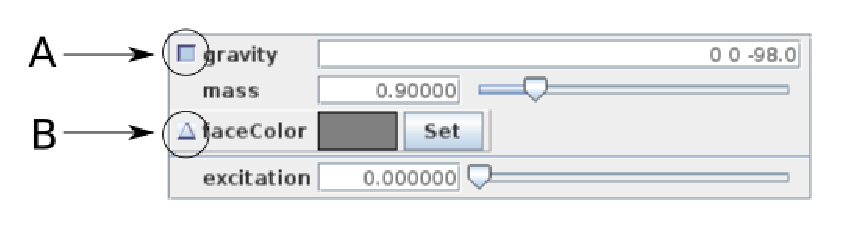
\includegraphics[]{images/controlPanelAnnotated}
\else
 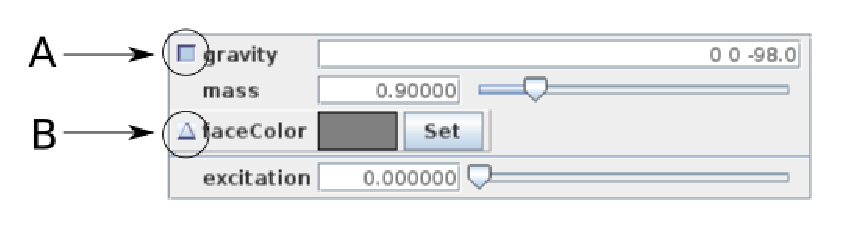
\includegraphics[width=4.5in]{images/controlPanelAnnotated}
\fi
\end{center}
\caption{Control panel created by the model {\tt SimpleMuscleWithPanel}.
Each of the property widgets consists of a text label followed by a
field displaying the property's value. A and B identify the icons for
the inheritable properties {\sf gravity} and {\sf faceColor},
indicating whether their values have has been explicitly set (A) or
inherited from an ancestor component (B).}
\label{controlPanel:fig}
\end{figure}

As described in Section \ref{CompositeInheritableProperties:sec}, some
properties are {\it inheritable}, meaning that their values can either
be set explicitly within their host component, or inherited from the
equivalent property in an ancestor component. Widgets for inheritable
properties include an icon in the left margin indicating whether the
value is explicitly set (square icon) or inherited from an ancestor
(triangular icon) (Figure \ref{controlPanel:fig}). These settings can
be toggled by clicking on the icon. Changing an {\it explicit} setting
to {\it inherited} will cause the property's value to be changed to
that of the nearest ancestor component, or to the property's default
value if no ancestor component contains an equivalent property.

% SimpleMuscleWithPanel

\subsection{Example: Controlling properties in multiple components}
\label{PropForMultComps:sec}

\begin{figure}[th]
\begin{center}
\iflatexml
 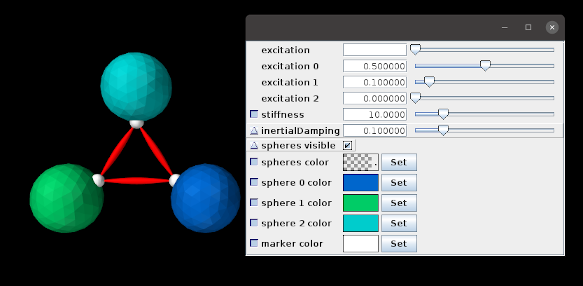
\includegraphics[]{images/ControlPanelDemo}
\else
 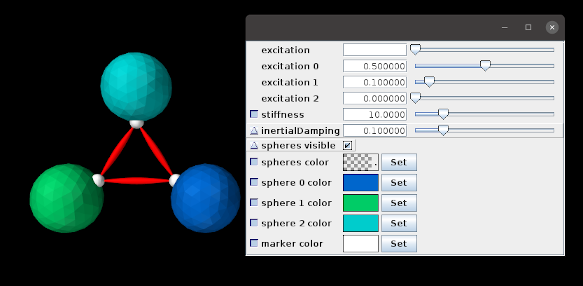
\includegraphics[width=6in]{images/ControlPanelDemo}
\fi
\end{center}
\caption{Model and control panel created by {\tt
ControlPanelDemo}.}
\label{controlPanelDemo:fig}
\end{figure}

It is sometimes useful to create a property widget that adjusts the
same property across several different components at the same time.
This can be done using the {\tt addWidget()} methods that accept
multiple hosts. An application model demonstrating this is defined in
%
\begin{verbatim}
  artisynth.demos.tutorial.ControlPanelDemo
\end{verbatim}
%
and shown in Figure \ref{controlPanelDemo:fig}.  The model creates a
simple arrangement of three spheres, connected by point-to-point
muscles and with collisions enabled
(Chapter \ref{ContactAndCollision:sec}), whose dynamic behavior can be
adjusted using the control panel. Selected rendering properties can
also be changed using the panel.  The class definition, excluding {\tt
include} statements, is shown below:
%
\lstset{numbers=left} 
\iflatexml
%% Hack: latexml lstinputlisting doesn't handle firstline correctly
\lstset{firstnumber={-20}}
\lstinputlisting[firstline=1]{../../src/artisynth/demos/tutorial/ControlPanelDemo.java}
\lstset{firstnumber={1}}
\else
\lstinputlisting[firstline=22]{../../src/artisynth/demos/tutorial/ControlPanelDemo.java}
\fi
\lstset{numbers=none}
%
First, a {\tt MechModel} is created with zero gravity and a default
{\sf inertialDamping} of 0.1 (lines 18-21). Next, three spheres are
created, each with a different color and a frame marker attached to
the top. These are positioned around the world coordinate origin, and
oriented with their tops pointing toward the origin (lines 26-47),
allowing them to be connected, via their markers, with three simple
muscles (lines 49-52) created using the support method {\tt
attachMuscle()} (lines 8-14). Collisions
(Chapter \ref{ContactAndCollision:sec}) are then enabled between all
spheres (line 55).

At lines 62-64, we explicitly set the render properties for each
marker; this is done because marker render properties are {\tt null}
by default and hence need to be explicitly set to enable widgets to be
created for them, as discussed further below.

Finally, a control panel is created for various dynamic and rendering
properties. These include the {\sf excitation} and material {\sf
stiffness} for all muscles (lines 71 and 75); the {\sf
inertialDamping}, rendering {\sf visibility} and {\sf faceColor} for
all spheres (lines 77, 79, and 81); and the rendering {\sf pointColor}
for all markers (lines 85). The panel also allows muscle excitations
and sphere face colors to be set individually (lines 72-74 and 82-84).
Some of the {\tt addWidget()} calls explicitly set the label text for
their widgets. For example, those controlling individual muscle
excitations are labeled as ``{\tt excitation 0}'', ``{\tt excitation
1}'', and ``{\tt excitation 2}'' to denote their associated muscle.

Some widgets are created for subproperties of their components (e.g.,
{\sf material.stiffness} and {\sf renderProps.faceColor}). The
following caveats apply in these cases:

\begin{enumerate}

\item The parent property (e.g., {\sf renderProps} for 
{\sf renderProps.faceColor}) must be present in the component.  While
this will generally be true, in some instances the parent property may
have a default value of {\tt null}, and must be explicitly set to a
non-{\tt null} value before the widget is created (otherwise the
subproperty will not be found and the widget creation will fail). This
most commonly occurs for the {\tt renderProps} property of smaller
components, like particles and markers; in the example, render
properties are explicitly assigned to the markers at lines 62-64.

\item If the parent property is {\it changed} for a particular
host, then the widget will no longer be able to access the
subproperty.  For instance, in the example, if the {\sf material}
property for a muscle is changed (via either code or the GUI), then
the widget controlling {\sf material.stiffness} will no longer be
able to access the {\sf stiffness} subproperty for that muscle.

\end{enumerate}

To run this example in ArtiSynth, select {\sf All demos > tutorial >
ControlPanelDemo} from the {\sf Models} menu. When the model is run,
the spheres will start to be drawn together by the muscles' intrinsic
stiffness.  Setting non-zero excitation values in the control panel
will increase the attraction, while setting stiffness values will
likewise affect the dynamics. The panel can also be used to make all
the spheres invisible, or to change their colors, either separately or
collectively.

\begin{sideblock}
When a single widget is used to control a property across multiple
host components, the property's value may not be the same for those
components. When this occurs, the widget's value field displays either
blank space (for numeric, string and enum values), a ``?'' (for
boolean values), or a checked pattern (for color values).  This is
illustrated in Figure \ref{controlPanelDemo:fig} for the ``{\tt
excitation}'' and ``{\tt spheres color}'' widgets, since their
individual values differ.
\end{sideblock}

\section{Custom properties}
\label{CustomProperties:sec}

Because of the usefulness of properties in creating control panels and
probes (Sections \ref{ControlPanels:sec}) and Section
\ref{Probes:sec}), model developers may wish to add their own
properties, either to the root model, or to a custom component.

This section provides only a brief summary of how to define
properties. Full details are available in the ``Properties'' section of
the \artisynthManual{maspack}{Maspack Reference Manual}.

\subsection{Adding properties to a component}

As mentioned in Section \ref{Properties:sec}, properties are
class-specific, and are exported by a class through code contained in
the class's definition.  Often, it is convenient to add properties to
the {\tt RootModel} subclass that defines the application model. In
more advanced applications, developers may want to add properties to a
custom component.

The property definition steps are:

\begin{description}

\item[Declare the property list:]\mbox{}

The class exporting the properties creates its own static instance of
a \javaclass[maspack.properties]{PropertyList}, using a declaration
like
%
\begin{lstlisting}[]
   static PropertyList myProps = new PropertyList (MyClass.class, MyParent.class);

   @Override   
   public PropertyList getAllPropertyInfo() {
      return myProps;
   }  
\end{lstlisting}
%
where {\tt MyClass} and {\tt MyParent} specify the class types of the
exporting class and its parent class. The {\tt PropertyList}
declaration creates a new property list, with a copy of all the
properties contained in the parent class.  If one does {\it not} want
the parent class properties, or if the parent class does not have
properties, then one would use the constructor
\javamethodAlt{maspack.properties.PropertyList.PropertyList(Class)}%
{PropertyList(MyClass.class)} instead. If the parent class is an
ArtiSynth model component (including the {\tt RootModel}), then it
will always have its own properties. The declaration of the method
{\tt getAllPropertyInfo()} exposes the property list to other classes.

\item[Add properties to the list:]\mbox{}

Properties can then be added to the property list, by calling the {\tt
PropertyList}'s
\javamethod*[maspack.properties.PropertyList]{add(String,String,Object)}
method:
% method table
\begin{lstlisting}[]
   PropertyDesc add (String name, String description, Object defaultValue);
\end{lstlisting}
%
where {\tt name} contains the name of the property, {\tt description}
is a comment describing the property, and {\tt defaultValue} is an
object containing the property's default value.  This is done inside a
static code block:
%
\begin{lstlisting}[]
   static {
      myProps.add ("stiffness", "spring stiffness", /*defaultValue=*/1);
      myProps.add ("damping", "spring damping", /*defaultValue=*/0);
   }
\end{lstlisting}
%
Variations on the {\tt add()} method exist for adding {\it read-only}
or {\it inheritable} properties, or for setting various property
options. Other methods allow the property list to be edited.

\item[Declare property accessor functions:]\mbox{}

For each property {\tt propXXX} added to the property list, accessor methods of
the form
%
\begin{lstlisting}[]
   void setPropXXX (TypeX value) {
      ...
   }

   TypeX getPropXXX() {
      TypeX value = ...
      return value;
   }
\end{lstlisting}
%
must be declared, where {\tt TypeX} is the value associated with the
property. 
\begin{sideblock}
It is possible to specify different names for the accessor functions
in the string argument {\tt name} supplied to the {\tt add()}
method. Read-only properties only require a {\it get} accessor.
\end{sideblock}

\end{description}

\subsection{Example: a visibility property}
%
An model illustrating the exporting of properties is defined in
%
\begin{verbatim}
  artisynth.demos.tutorial.SimpleMuscleWithProperties
\end{verbatim}
%
This model extends {\tt SimpleMuscleWithPanel} (Section
\ref{SimpleMuscleExample:sec}) to provide a custom property
{\tt boxVisible} that is added to the control panel.
The class definition, excluding {\tt include} statements,
is shown below:
%
\lstset{numbers=left}
\begin{lstlisting}[]
public class SimpleMuscleWithProperties extends SimpleMuscleWithPanel {

   // internal property list; inherits properties from SimpleMuscleWithPanel
   static PropertyList myProps =
      new PropertyList (
         SimpleMuscleWithProperties.class, SimpleMuscleWithPanel.class);

   // override getAllPropertyInfo() to return property list for this class
   public PropertyList getAllPropertyInfo() {
      return myProps;
   }

   // add new properties to the list
   static {
      myProps.add ("boxVisible", "box is visible", false);
   }

   // declare property accessors
   public boolean getBoxVisible() {
      return box.getRenderProps().isVisible();
   }

   public void setBoxVisible (boolean visible) {
      RenderProps.setVisible (box, visible);
   }

   public void build (String[] args) throws IOException {

      super.build (args);

      panel.addWidget (this, "boxVisible");
      panel.pack();
   }
}
\end{lstlisting}
\lstset{numbers=none}
%
First, a property list is created for the application class {\tt
SimpleMuscleWithProperties.class} which contains a copy of all the
properties from the parent class {\tt SimpleMuscleWithPanel.class}
(lines 4-6). This property list is made visible by overriding {\tt
getAllPropertyInfo()} (lines 9-11). The {\tt boxVisible} property
itself is then added to the property list (line 15), and accessor
functions for it are declared (lines 19-25).

\begin{figure}[t]
\begin{center}
\iflatexml
 \includegraphics[]{images/boxVisiblePanel}
\else
 \includegraphics[width=3in]{images/boxVisiblePanel}
\fi
\end{center}
\caption{Control panel created by the model {\tt SimpleMuscleWithProperties},
showing the newly defined property {\tt boxVisible}.}
\label{boxVisiblePanel:fig}
\end{figure}

The {\tt build()} method calls {\tt super.build()} to perform all the
model creation required by the super class, and then adds an
additional widget for the {\tt boxVisible} property to the control
panel.

To run this example in ArtiSynth, select {\sf All demos > tutorial >
SimpleMuscleWithProperties} from the {\sf Models} menu. The control
panel will now contain an additional widget for the property {\tt
boxVisible} as shown in Figure \ref{boxVisiblePanel:fig}. Toggling
this property will make the box visible or invisible in the viewer.

% SimpleMuscleWithProperties

\section{Controllers and monitors}
\label{ControllersAndMonitors:sec}

Application models can define custom {\it controllers} and {\it
monitors} to control input values and monitor output values as a
simulation progresses. Controllers are called every time step
immediately before the {\tt advance()} method, and monitors are called
immediately after (Section \ref{ModelAdvancement:sec}).  An example of
controller usage is provided by ArtiSynth's inverse modeling feature,
which uses an internal controller to estimate the actuation signals
required to follow a specified motion trajectory.

More precise details about controllers and monitors and how they
interact with model advancement are given in the
\artisynthManual{artisynth}{ArtiSynth Reference Manual}.

\subsection{Implementation}
\label{ControllerImplementation:sec}

Applications may declare whatever controllers or monitors they require
and then add them to the root model using the methods
\javamethod*[artisynth.core.workspace.RootModel]{addController()} and
\javamethod*[artisynth.core.workspace.RootModel]{addMonitor()}.
They can be any type of
\javaclass[artisynth.core.modelbase]{ModelComponent} that implements
the \javaclass[artisynth.core.modelbase]{Controller} or
\javaclass[artisynth.core.modelbase]{Monitor} interfaces.  For
convenience, most applications simply subclass
the default implementations
\javaclass[artisynth.core.modelbase]{ControllerBase} or
\javaclass[artisynth.core.modelbase]{MonitorBase} and then override
the necessary methods.

The primary methods associated with both controllers and
monitors are:
% method table
\begin{lstlisting}[]
  public void initialize (double t0);

  public void apply (double t0, double t1);

  public boolean isActive();
\end{lstlisting}
%
{\tt apply(t0, t1)} is the ``business'' method and is called once per
time step, with {\tt t0} and {\tt t1} indicating the start and end
times $t_0$ and $t_1$ associated with the step.  {\tt initialize(t0)}
is called whenever an application model's state is set (or reset) at a
particular time $t_0$. This occurs when a simulation is first started
or after it is reset (with $t_0 = 0$), and also when the state is
reset at a waypoint or during adaptive stepping.

{\tt isActive()} controls whether a controller or monitor is active;
if {\tt isActive()} returns {\tt false} then the {\tt apply()} method
will not be called.
The default implementations
\javaclass[artisynth.core.modelbase]{ControllerBase} and
\javaclass[artisynth.core.modelbase]{MonitorBase}, via their
superclass \javaclass[artisynth.core.modelbase]{ModelAgentBase}, also
provide a {\tt setActive()} method to control this setting, and export
it as the property {\sf active}. This allows controller and monitor
activity to be controlled at run time.

\begin{sideblock}
To enable or disable a controller or monitor at run time, locate it in
the navigation panel (under the RootModel's {\sf controllers} or {\sf
monitors} list), chose {\sf Edit properties ...} from the right-click
context menu, and set the {\sf active} property as desired.
\end{sideblock}

Controllers and monitors may be associated with a particular model
(among the list of models owned by the root model). This model may be
set or queried using
% method table
\begin{lstlisting}[]
  void setModel (Model m);

  Model getModel();
\end{lstlisting}
%
If associated with a model, {\tt apply()} will be called immediately
before (for controllers) or after (for monitors) the model's {\tt
advance()} method. If not associated with a model, then {\tt apply()}
will be called before or after the advance of {\it all} the models
owned by the root model.

Controllers and monitors may also contain {\it state}, in which case
they should implement the relevant methods from the
\javaclass[artisynth.core.modelbase]{HasState} interface.

Typical actions for a controller include setting input forces or
excitation values on components, or specifying the motion trajectory
of parametric components (Section \ref{DynamicVsParametric:sec}).
Typical actions for a monitor include observing or recording
the motion profiles or constraint forces that arise
from the simulation.

\subsubsection{Target positions and velocities}
\label{targetPositions:sec}

When setting the position and/or velocity of a dynamic component that has been
set to be parametric (Section \ref{DynamicVsParametric:sec}), a controller can
opt to set its position and/or velocity directly. However, it is often preferable
to instead set the component's {\it target position} and/or {\it target
velocity}, since this allows the solver to properly interpolate the position
and velocity during the time step. 

Whereas setting a position has no effect on velocity and vice versa, setting
target positions and velocities {\it does} account for the coupling between the
two. Specifically,

\begin{itemize}

\item If a target position is set and the target velocity is {\it not} set,
then during simulation the component's position will be set to the target
position and its velocity will be determined by {\it differentiating} the
target position (albeit with a one-step time lag).

\item If a target velocity is set and the target position is {\it not} set,
then during simulation the component's velocity will be set to the target
velocity and its position will be set by {\it integrating} the target velocity.

\item If {\it both} target position and target velocity are set (which is not
commonly done), then during simulation both with be used to update the
component's position and velocity.
	
\end{itemize}

For \javaclass[artisynth.core.mechmodels]{Point}-based components,
target positions and velocities are exported as the properties {\sf
targetPosition} and {\sf targetVelocity}, with the accessors:
%
% method table
\begin{lstlisting}[]
  setTargetPosition (Point3d pos);
  Point3d getTargetPosition ();       // read-only

  setTargetVelocity (Vector3d vel);
  Vector3d getTargetVelocity ();      // read-only
\end{lstlisting}
%
For \javaclass[artisynth.core.mechmodels]{Frame}-based components, target
positions and velocities are exported as the properties {\sf targetPosition},
{\sf targetOrientation} and {\sf targetVelocity}, with the accessors:
% method table
\begin{lstlisting}[]
  setTargetPosition (Point3d pos);
  setTargetOrientation (AxisAngle axisAng);
  setTargetPose (RigidTransform3d TFW);
  Point3d getTargetPosition ();       // read-only
  AxisAngle getTargetOrientation ();  // read-only
  RigidTransform3d getTargetPose();   // read-only

  setTargetVelocity (Twist vel);
  Twist getTargetVelocity ();         // read-only
\end{lstlisting}
%

\subsection{Example: A controller to move a point}

A model showing an application-defined controller is defined in
%
\begin{verbatim}
  artisynth.demos.tutorial.SimpleMuscleWithController
\end{verbatim}
%
This simply extends {\tt SimpleMuscle} (Section
\ref{SimpleMuscleExample:sec}) and adds a controller which moves the
fixed particle {\tt p1} along a circular path.  The complete class
definition is shown below:
%
\lstset{numbers=left}
\lstinputlisting{../../src/artisynth/demos/tutorial/SimpleMuscleWithController.java}
\lstset{numbers=none}
%
A controller called {\tt PointMover} is defined by extending {\tt
ControllerBase} and overriding the {\tt apply()} method. It stores the
point to be moved in {\tt myPnt}, and the initial position in
{\tt myPos0}. The {\tt apply()} method computes a target position for
the point that starts at {\tt myPos0} and then moves in a circle in the
$z$-$x$ plane with an angular velocity of $\pi/2$ rad/sec (lines 22-28).

The {\tt build()} method calls {\tt super.build()} to create the model
used by {\tt SimpleMuscle}, and then creates an instance of {\tt
PointMover} to move particle {\tt p1} and adds it to the root model
(line 34). The viewer bounds are updated to make the circular motion
more visible (line 36).

To run this example in ArtiSynth, select {\sf All demos > tutorial >
SimpleMuscleWithController} from the {\sf Models} menu. When
the model is run, the fixed particle {\tt p1} will trace
out a circular path in the $z$-$x$ plane.

\section{Probes}
\label{Probes:sec}

In addition to controllers and monitors, applications can also attach
streams of data, known as {\it probes}, to input and output values
associated with the simulation. Probes derive from the same base class
\javaclass[artisynth.core.modelbase]{ModelAgentBase} as 
controllers and monitors, 
but differ in that 

\begin{enumerate}

\item They are associated with an explicit time interval during which
they are applied;

\item They can have an attached file for supplying input data or
recording output data;

\item They are displayable in the ArtiSynth {\it timeline} panel.

\end{enumerate}

A probe is applied (by calling its {\tt apply()} method) only for time
steps that fall within its time interval. This interval can be set and
queried using the following methods:
% method table
\begin{lstlisting}[]
   setStartTime (double t0);
   setStopTime (double t1);
   setInterval (double t0, double t1);
 
   double getStartTime();
   double getStopTime();
\end{lstlisting}
%
The probe's attached file can be set and queried using:
% method table
\begin{lstlisting}[]
   setAttachedFileName (String filePath);
   String getAttachedFileName ();
\end{lstlisting}
%
where {\tt filePath} is a string giving the file's path name.  If {\tt
filePath} is relative (i.e., it does not start at the file system root), then
it is assumed to be relative to the {\it ArtiSynth working folder}, which
can be queried and set using the methods
%
\begin{lstlisting}[]
   File ArtisynthPath.getWorkingFolder();
   ArtisynthPath.setWorkingFolder (File folder);
\end{lstlisting}
%
of \javaclass[artisynth.core.util]{ArtisynthPath}.
The working folder can also be set from the ArtiSynth GUI
by choosing {\sf File > Set working folder ...}.
\begin{sideblock}
If not explicitly set within the application, the working folder will default
to a system dependent setting, which may be the user's home folder, or the
working folder of the process used to launch Artisynth.
\end{sideblock}

Details about the timeline display can be found in
the section ``The Timeline'' in the
\artisynthManual{uiguide}{ArtiSynth User Interface Guide}.

There are two types of probe: {\it input probes}, which are applied at
the beginning of each simulation step before the controllers, and {\it
output probes}, which are applied at the end of the step after the
monitors.

While applications are free to construct any type of probe by
subclassing either \javaclass[\probes]{InputProbe} or
\javaclass[\probes]{OutputProbe}, most applications
utilize either \javaclass[\probes]{NumericInputProbe} or
\javaclass[\probes]{NumericOutputProbe}, which
explicitly implement streams of numeric data which are connected to
properties of various model components.  The remainder of this section
will focus on numeric probes.

As with controllers and monitors, probes also implement a {\tt
isActive()} method that indicates whether or not the probe is active.
Probes that are not active are not invoked. Probes also provide a
{\tt setActive()} method to control this setting, and export it as the
property {\sf active}. This allows probe activity to be controlled at
run time.

\begin{sideblock}
To enable or disable a probe at run time, locate it in the navigation
panel (under the RootModel's {\sf inputProbes} or {\sf outputProbes}
list), chose {\sf Edit properties ...} from the right-click context
menu, and set the {\sf active} property as desired.

Probes can also be enabled or disabled in the timeline, by either
selecting the probe and invoking {\sf activate} or {\sf deactivate}
from the right-click context menu, or by clicking the track {\sf mute}
button (which activates or deactivates all probes on that track).
\end{sideblock}

\subsection{Numeric probe structure}
\label{NumericProbeStructure:sec}

Numeric probes are associated with:

\begin{itemize}

\item {\it A vector of temporally-interpolated numeric data};

\item {\it One or more properties} to which the probe is bound and
which are either set by the numeric data (input probes), or used to
set the numeric data (output probes).

\end{itemize}

The numeric data is implemented internally by a
\javaclass[maspack.interpolation]{NumericList}, which stores the data
as a series of vector-valued knot points at prescribed times $t_k$ and
then interpolates the data for an arbitrary time $t$ using an
interpolation scheme provided by
\javaclass[maspack.interpolation]{Interpolation}.

Some of the numeric probe methods associated with the interpolated
data include:
% method table
\begin{lstlisting}[]
   int getVsize();                      // returns the size of the data vector
   setInterpolationOrder (Order order); // sets the interpolation scheme
   Order getInterpolationOrder();       // returns the interpolation scheme

   VectorNd getData (double t);         // interpolates data for time t
   NumericList getNumericList();        // returns the underlying NumericList
\end{lstlisting}
%
Interpolation schemes are described by the enumerated type {\tt
Interpolation.Order} and presently include:

\begin{description}

\item[Step]\mbox{}

Values at time $t$ are set to the values of the closest knot point
$k$ such that $t_k \le t$.

\item[Linear]\mbox{}

Values at time $t$ are set by linear interpolation of the knot points
$(k, k+1)$ such that $t_k \le t \le t_{k+1}$.

\item[Parabolic]\mbox{}

Values at time $t$ are set by quadratic interpolation of the knots
$(k-1, k, k+1)$ such that $t_k \le t \le t_{k+1}$.

\item[Cubic]\mbox{}

Values at time $t$ are set by cubic Catmull interpolation of the knots
$(k-1, \ldots, k+2)$ such that $t_k \le t \le t_{k+1}$.

\end{description}

Each property bound to a numeric probe must have a value
that can be mapped onto a scalar or vector value. Such properties
are know as {\it numeric properties}, and whether or not
a value is numeric can be tested using\pdfbreak
\javamethodAlt{maspack.properties.NumericConverter.isNumeric()}%
{NumericConverter.isNumeric(value)}.

By default, the total number of scalar and vector values associated
with all the properties should equal the size of the interpolated
vector (as returned by
\javamethod*[\probes.NumericProbeBase]{getVsize()}).
However, it is possible to establish more complex mappings between the
property values and the interpolated vector. These mappings are beyond
the scope of this document, but are discussed in the sections ``General
input probes'' and ``General output probes'' of the
\artisynthManual{uiguide}{ArtiSynth User Interface Guide}.

\subsection{Creating probes in code}

This section discusses how to create numeric probes in code.  They can
also be created and added to a model graphically, as described in the
section ``Adding and Editing Numeric Probes'' in the
\artisynthManual{uiguide}{ArtiSynth User Interface Guide}.

Numeric probes have a number of constructors and methods that make it
relatively easy to create instances of them in code. For 
\javaclass[\probes]{NumericInputProbe}, there
is the constructor
% method table
\begin{lstlisting}[]
   NumericInputProbe (ModelComponent c, String propPath, String filePath);
\end{lstlisting}
%
which creates a {\tt NumericInputProbe}, binds it to a property
located relative to the component {\tt c} by {\tt propPath}, and then
attaches it to the file indicated by {\tt filePath} and loads data
from this file (see Section \ref{DataFileFormat:sec}). The probe's start and
stop times are specified in the file, and its vector size is
set to match the size of the scalar or vector value associated with
the property.

To create a probe attached to multiple properties, one may use the
constructor
% method table
\begin{lstlisting}[]
   NumericInputProbe (ModelComponent c, String propPaths[], String filePath);
\end{lstlisting}
%
which binds the probe to multiple properties specified relative to
{\tt c} by {\tt propPaths}. The probe's vector size is set to
the sum of the sizes of the scalar or vector values associated with
these properties.

For \javaclass[\probes]{NumericOutputProbe}, one may use
the constructor
% method table
\begin{lstlisting}[]
   NumericOutputProbe (ModelComponent c, String propPath, String filePath, double interval);
\end{lstlisting}
%
which creates a {\tt NumericOutputProbe}, binds it to the property
{\tt propPath} located relative to {\tt c}, and then attaches it to
the file indicated by {\tt filePath}. The argument {\tt interval}
indicates the {\it update interval} associated with the probe, in seconds;
a value of 0.01 means that data will be added to the probe every 0.01
seconds.  If {\tt interval} is specified as -1, then the update interval
will default to the simulation step size. This interval can
also be accessed after the probe is created using
% method table
\begin{lstlisting}[]
   int getUpdateInterval()              // returns the update interval
   void setUpdateInterval(int sec)      // sets the update interval (seconds)
\end{lstlisting}[]
%
To create an output probe attached to multiple properties, one may use the
constructor
% method table
\begin{lstlisting}[]
   NumericOutputProbe (
      ModelComponent c, String propPaths[], String filePath, double interval);
\end{lstlisting}
%

\begin{sideblock}
As the simulation proceeds, an output probe will accumulate data, but
this data will not be saved to any attached file until the probe's
{\tt save()} method is called. This can be requested in the GUI for
all probes by clicking on the {\sf Save} button in the timeline
toolbar, or for specific probes by selecting them in the navigation
panel (or the timeline) and then choosing {\sf Save data} in the
right-click context menu.
\end{sideblock}

Output probes created with the above constructors have a default
interval of [0, 1]. A different interval may be set using
{\tt setInterval()}, {\tt setStartTime()}, or {\tt setStopTime()}.

\subsection{Example: probes connected to SimpleMuscle}
\label{SimpleMuscleWithProbes:sec}

A model showing a simple application of probes is defined in
%
\begin{verbatim}
  artisynth.demos.tutorial.SimpleMuscleWithProbes
\end{verbatim}
%
This extends {\tt SimpleMuscle} (Section
\ref{SimpleMuscleExample:sec}) to add an input probe to move particle
{\tt p1} along a defined path, along with an output probe to record
the velocity of the frame marker.  The complete class definition is
shown below:
%
\lstset{numbers=left}
\lstinputlisting{../../src/artisynth/demos/tutorial/SimpleMuscleWithProbes.java}
\lstset{numbers=none}
%
The input and output probes are added using the custom methods {\tt
createInputProbe()} and {\tt createOutputProbe()}. At line 14, {\tt
createInputProbe()} creates a new input probe bound to the {\tt
targetPosition} property for the component {\tt particles/p1} located
relative to the {\tt MechModel} {\tt mech}. The same constructor
attaches the probe to the file\pdfbreak{\tt simpleMuscleP1Pos.txt}, which is
read to load the probe data. The format of this and other probe data
files is described in Section \ref{DataFileFormat:sec}.  The method
\javamethod*[maspack.util]{PathFinder.getSourceRelativePath()}
is used to locate the file relative to the source directory for the
application model (see Section
\ref{PathFinder:sec}). The probe is then given the name {\tt "Particle
Position"} (line 18) and added to the root model (line 19).

Similarly, {\tt createOutputProbe()} creates a new output probe which
is bound to the {\tt velocity} property for the component {\tt
particles/0} located relative to {\tt mech}, is attached to the file {\tt
simpleMuscleMkrVel.txt} located in the application model source
directory, and is assigned an update interval of 0.01 seconds. This probe is
then named {\tt "FrameMarker Velocity"} and added to the root model.

The {\tt build()} method calls {\tt super.build()} to create
everything required for {\tt SimpleMuscle}, calls {\tt
createInputProbe()} and {\tt createOutputProbe()} to add the probes,
and adjusts the {\tt MechModel} viewer bounds to make the resulting
probe motion more visible.

To run this example in ArtiSynth, select {\sf All demos > tutorial >
SimpleMuscleWithProbes} from the {\sf Models} menu. After the model is
loaded, the input and output probes should appear on the timeline
(Figure \ref{probes:fig}). Expanding the probes should display their
numeric contents, with the knot points for the input probe clearly
visible.  Running the model will cause particle {\tt p1} to trace the
trajectory specified by the input probe, while the velocity of the
marker is recorded in the output probe. Figure
\ref{probesExpanded:fig} shows an expanded view of both probes after
the simulation has run for about six seconds.

% SimpleMuscleWithProbes

\begin{figure}[ht]
\begin{center}
\iflatexml
 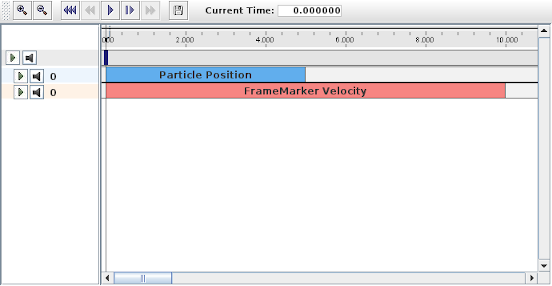
\includegraphics[]{images/timelineProbes}
\else
 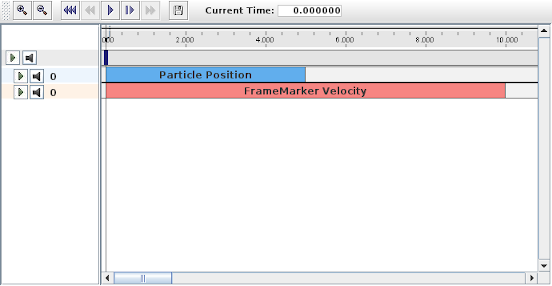
\includegraphics[width=4in]{images/timelineProbes}
\fi
\end{center}
\caption{Timeline view of the probes created by SimpleMuscleWithProbes.}
\label{probes:fig}
\end{figure}

\begin{figure}[ht]
\begin{center}
\iflatexml
 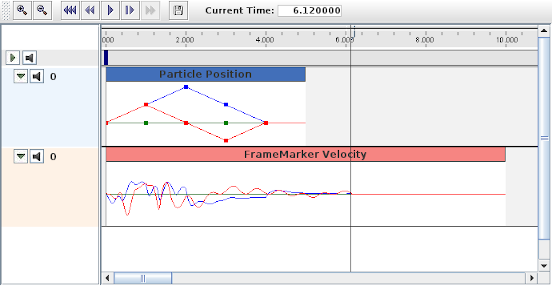
\includegraphics[]{images/timelineProbesExpanded}
\else
 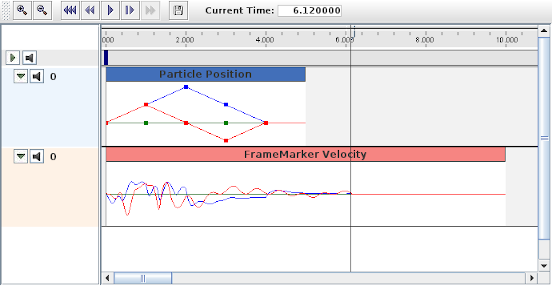
\includegraphics[width=4in]{images/timelineProbesExpanded}
\fi
\end{center}
\caption{Expanded view of the probes after {\tt
SimpleMuscleWithProbes} has run for about 6 seconds, showing the data
accumulated in the output probe {\tt "FrameMarker Velocity"}.}
\label{probesExpanded:fig}
\end{figure}

\subsection{Data file format}
\label{DataFileFormat:sec}

The data files associated with numeric probes are ASCII files
containing two lines of header information followed by a set of knot
points, one per line, defining the numeric data. The time value
(relative to the probe's start time) for each knot point can be
specified explicitly at the start of the each line, in which case the
file takes the following format:
%
\begin{lstlisting}[]
startTime stopTime scale
interpolation vsize explicit
t0 val00 val01 val02 ...
t1 val10 val11 val12 ...
t0 val20 val21 val22 ...
...
\end{lstlisting}
%
Knot point information begins on line 3, with each line being a
sequence of numbers giving the knot's time followed by $n$ values,
where $n$ is the vector size of the probe (i.e., the value returned by
{\tt getVsize()}).

Alternatively, time values can be implicitly specified starting at 0
(relative to the probe's start time) and incrementing by a uniform
{\tt timeStep}, in which case the file assumes a second format:
%
\begin{lstlisting}[]
startTime stopTime scale
interpolation vsize timeStep
val00 val01 val02 ...
val10 val11 val12 ...
val20 val21 val22 ...
...
\end{lstlisting}
%
For both formats, {\tt startTime}, {\tt startTime}, and {\tt scale}
are numbers giving the probe's start and stop time in seconds and {\tt
scale} gives the scale factor (which is typically 1.0).  {\tt
interpolation} is a word describing how the data should be
interpolated between knot points and is the string value of {\tt
Interpolation.Order} as described in Section
\ref{NumericProbeStructure:sec} (and which is typically {\tt Linear},
{\tt Parabolic}, or {\tt Cubic}). {\tt vsize} is an integer giving the
probe's vector size.

The last entry on the second line is either a number specifying a
(uniform) time step for the knot points, in which case the file
assumes the second format, or the keyword {\tt explicit}, in which
case the file assumes the first format.

As an example, the file used to specify data for the input probe in
the example of Section \ref{SimpleMuscleWithProbes:sec} looks like
the following:
%
\begin{lstlisting}[]
0 4.0 1.0
Linear 3 explicit
0.0  0.0 0.0 0.0 
1.0  0.5 0.0 0.5
2.0  0.0 0.0 1.0
3.0 -0.5 0.0 0.5
4.0  0.0 0.0 0.0
\end{lstlisting}
%
Since the data is uniformly spaced beginning at 0, it would also be
possible to specify this using the second file format:
%
\begin{lstlisting}[]
0 4.0 1.0
Linear 3 1.0
 0.0 0.0 0.0 
 0.5 0.0 0.5
 0.0 0.0 1.0
-0.5 0.0 0.5
 0.0 0.0 0.0
\end{lstlisting}
%

\subsection{Adding input probe data in code}
\label{probeDataInCode:sec}

It is also possible to specify input probe data directly in code,
instead of reading it from a file. For this, one would use the
constructor
% method table
\begin{lstlisting}[]
   NumericInputProbe (ModelComponent c, String propPath, double t0, double t1)
\end{lstlisting}
%
which creates a {\tt NumericInputProbe} with the specified property
and with start and stop times indicated by {\tt t0} and {\tt t1}.
Data can then be added to this probe using the method
% method table
\begin{lstlisting}[]
   addData (double[] data, double timeStep)
\end{lstlisting}
%
where {\tt data} is an array of knot point data. This contains the
same knot point information as provided by a file (Section
\ref{DataFileFormat:sec}), arranged in row-major order.  Times values
for the knots are either implicitly specified, starting at 0 (relative
to the probe's start time) and increasing uniformly by the amount
specified by {\tt timeStep}, or are explicitly specified at the
beginning of each knot if {\tt timeStep} is set to the built-in
constant {\tt NumericInputProbe.EXPLICIT\_TIME}. The size of the {\tt
data} array should then be either $n*m$ (implicit time values) or
$(n+1)*m$ (explicit time values), where $n$ is the probe's vector size
and $m$ is the number of knots.

As an example, the data for the input probe in Section
\ref{SimpleMuscleWithProbes:sec} could have been specified
using the following code:
%
\begin{lstlisting}[]
      NumericInputProbe p1probe =
         new NumericInputProbe (
            mech, "particles/p1:targetPosition", 0, 5);
      p1probe.addData (
         new double[] {
            0.0,  0.0, 0.0, 0.0,
            1.0,  0.5, 0.0, 0.5,
            2.0,  0.0, 0.0, 1.0,
            3.0, -0.5, 0.0, 0.5,
            4.0,  0.0, 0.0, 0.0 },
            NumericInputProbe.EXPLICIT_TIME);
\end{lstlisting}

When specifying data in code, the interpolation defaults to {\tt
Linear} unless explicitly specified using\pdfbreak
{\tt setInterpolationOrder()}, as in, for example:
%
\begin{lstlisting}[]
   probe.setInterpolationOrder (Order.Cubic);
\end{lstlisting}
%

Data can also be added incrementally, using the method
%
\begin{lstlisting}[]
   probe.addData (double t, VectorNd values)
\end{lstlisting}
%
which adds a data knot the specified {\tt values} at time {\tt t}; {\tt values}
should have a size equal to the probe's vector size. For example, the
array-based example above could instead by implemented as
\begin{lstlisting}[]
      NumericInputProbe p1probe =
         new NumericInputProbe (
            mech, "particles/p1:targetPosition", 0, 5);
      p1probe.addData (0.0, new VectorNd (0.0, 0.0, 0.0));
      p1probe.addData (1.0, new VectorNd (0.5, 0.0, 0.5));
      p1probe.addData (2.0, new VectorNd (0.0, 0.0, 1.0));
      p1probe.addData (3.0, new VectorNd (-0.5, 0.0, 0.5));
      p1probe.addData (4.0, new VectorNd (0.0, 0.0, 0.0));
\end{lstlisting}

When an input probe is created {\it without} data specified in its constructor
(e.g., by means of a probe data file), then it automatically adds knot points
at its start and end times, with values set from the current values of its
bound properties. Applying such a probe, without adding additional data, will
thus leave the values of its properties unchanged.

The {\tt addData()} methods described above do not remove existing knot points
(although they will overwrite knots that exist at the same times). In
order to {\tt replace} all data, one can first call the method
%
\begin{lstlisting}[]
   probe.clearData()
\end{lstlisting}
%
which removes all knot points. Probes with no knots assign 0 to all their
property values.  Data can subsequently be added using the {\tt addData()}
methods. Alternatively, one can call 
% method table
\begin{lstlisting}[]
   setData (double[] data, double timeStep)
\end{lstlisting}
%
which behaves identically to the {\tt addData(double[],timeStep)} method
except that it first removes all existing data.

Another convenient way to add data to a probe is to simply copy it from another
probe, using the method
% method table
\begin{lstlisting}[]
   setValues (NumericProbeBase src, boolean useAbsoluteTime)
\end{lstlisting}
%
All knot points and values are copied from {\tt src}, which can be any numeric
probe (input or output), with the only restriction being that its vector size
must equal or exceed that of the calling probe (extra values are ignored).  If
{\tt useAbsoluteTime} is {\tt true}, time values are mapped between the probes
using absolute time; otherwise, probe relative time is used.  When using this
method, care should be taken to ensure that the there will be knot points to
cover the start and stop times of the calling probe.

\subsubsection{Extending data to the start and end}

By explicitly using the {\tt clearData()} or {\tt setData()} methods, it is
possible to create an input probe for which data is missing at its start and/or
stop times. The behavior in that case is determined by the probe's {\sf
extendData} property: if the property is set to {\tt true}, then data values
between the start time and the first knot, or the last knot and the stop time,
are set to the values of the first and last knot, respectively.  Otherwise,
these data values are set to zero.

As with all properties, {\sf extendData} can be set and queried in code using
the accessors
% method table
\begin{lstlisting}[]
   boolean getExtendData()
   void setExtendData (boolean enable)
\end{lstlisting}
%
The default value of {\sf extendData} is {\tt true}.  As mentioned above,
probes with no data set their data values uniformly to 0.

\subsection{Tracing probes}

\begin{figure}[ht]
\begin{center}
\iflatexml
 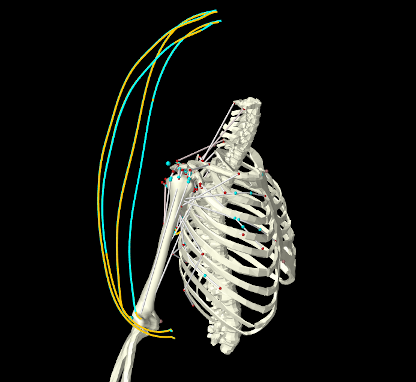
\includegraphics[]{images/shoulderTracing}
\else
 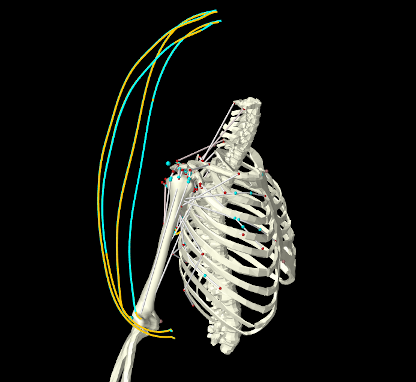
\includegraphics[width=3in]{images/shoulderTracing}
\fi
\end{center}
\caption{Tracing probes used to show the desired target (cyan)
and actual (gold) trajectories of some marker points attached near the elbow of
an ArtiSynth shoulder model undergoing an inverse simulation.}
\label{shoulderTracing:fig}
\end{figure}

It is often useful to follow the path or evolution of a position or vector
quantity as it evolves in time during a simulation. For example, one may wish
to trace out the path of some points, as per Figure \ref{shoulderTracing:fig},
which traces the actual and desired paths of some marker points during an
inverse simulation of the type described in
Chapter \ref{InverseSimulation:sec}.

ArtiSynth supplies \javaclass[\probes]{TracingProbe}s that can be used for this
purpose.  A tracing probe can be attached to any component that implements the
interface
\javaclass[\mbase]{Traceable}, for any of the properties that
are exported by its 
\javamethod[\mbase.Traceable]{getTraceables()} method.
At present, {\tt Traceable} is implemented for the following components:

\begin{description}

\item[\protect{\javaclass[\mech]{Point}}]\mbox{}

Traceable properties are {\sf point} and {\sf force}.

\item[\protect{\javaclass[\mech]{Frame}}]\mbox{}

Traceable properties are {\sf transforce} and {\sf moment}.

\end{description}

%\begin{center}
%\begin{tabular}{ll}
%\hline
%Component & tracable properties\\
%\hline
%\javaclass[\mech]{Point} & {\sf position}, {\sf force}\\
%\javaclass[\mech]{Frame} & {\sf transforec}, {\sf moment}\\
%\hline
%\end{tabular}
%\end{center}

Tracing probes are easily created using the {\tt RootModel} method
%
\begin{methodtable}{0.95}{0.05}
%
\methodentry
{artisynth.core.workspace.RootModel.addTracingProbe()}%
{TracingProbe addTracingProbe (Traceable comp, String propName,
double startTime, double stopTime)}%
{\ }%
%
\end{methodtable}
%
which produces a tracing probe of specified duration for the indicated
component and property name pair. During simulation, the probe will record the
desired property at the rate defined by its {\sf updateInterval}, and also
render it in the viewer. In cases where the probe renders all its stored values
(as with {\tt PointTracingProbe}s, described below), the interval at which this
occurs can be controlled by its {\sf renderInterval} property, accessed
in code via
%
\begin{methodtable}{0.5}{0.5}
%
\methodentry
{\probes.TracingProbe.getRenderInterval()}%
{double getRenderInterval()}%
{Return the render interval}%
%
\methodentry
{\probes.TracingProbe.getRenderInterval()}%
{void setRenderInterval(double interval)}%
{Set the render interval (seconds)}%
%
\end{methodtable}
%
Specifying a render interval of -1 (the default) will cause
the render interval to equal the update interval.

Two types of tracing probes are currently implemented:

\begin{description}

\item[\protect{\javaclass[\probes]{PointTracingProbe}}]\mbox{}

Created for point properties, this renders the path of the point position over
the duration of the probe, either as a continuous curve (if the probe's {\sf
pointTracing} property is {\tt false}, the default setting), or as discrete
points. The appearance of the rendering is controlled by subproperties of the
probe's render properties, using {\sf lineStyle}, {\sf lineRadius}, {\sf
lineWidth} and {\sf lineColor} (for continuous curves) or {\sf pointStyle},
{\sf pointRadius}, {\sf pointSize} and {\sf pointColor} (for points).

\item[\protect{\javaclass[\probes]{VectorTracingProbe}}]\mbox{}

Created for vector properties, this renders the vector quantity at the current
simulation time as a line segment anchored at the current position of the
component. The length of the line segment is controlled by the probe's {\sf
lengthScaling} property, and other aspects of the appearance are controlled by
the subproperties {\sf lineStyle}, {\sf lineRadius}, {\sf lineWidth} and {\sf
lineColor} of the probe's render properties. Vector tracing is mostly used to
visual instantaneous forces.

\end{description}

The following code fragment attaches a tracing probe to the last frame marker
of the {\tt MultiJointedArm} example of Section \ref{MultiJointedArm:sec}:
%
\begin{lstlisting}[]
import artisynth.core.probes.TracingProbe;
   ...
   FrameMarker mkr = myMech.frameMarkers().get(/*mkrIndex*/4);
   TracingProbe tprobe = addTracingProbe (mkr, "position", 0.0, 2.0);
   tprobe.setName ("marker trace");
   RenderProps.setLineColor (tprobe, Color.ORANGE);
\end{lstlisting}
%
with the results shown in Figure \ref{PointLineTracing:fig} (left).  To instead
render the output as points, and with a coarser render interval of 0.02, one
could modify the probe properties using
%
\begin{lstlisting}[]
import artisynth.core.probes.PointTracingProbe;
   ...
   ((PointTracingProbe)tprobe).setPointTracing (true);
   tprobe.setRenderInterval (0.02); // display points 0.02 sec apart
   RenderProps.setSphericalPoints(tprobe, 0.01, Color.GREEN);
\end{lstlisting}
%
with the results shown in Figure \ref{PointLineTracing:fig} (right).

\begin{figure}[h]
\begin{center}
\begin{tabular}{cc}
\iflatexml
 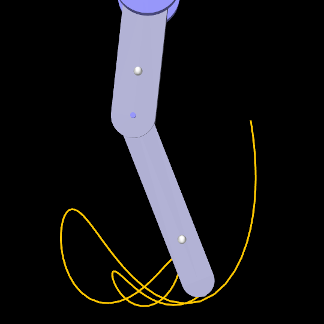
\includegraphics[]{images/LineTracing}
 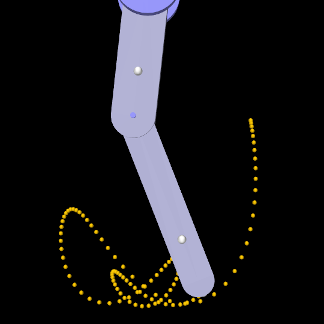
\includegraphics[]{images/PointTracing}
\else
 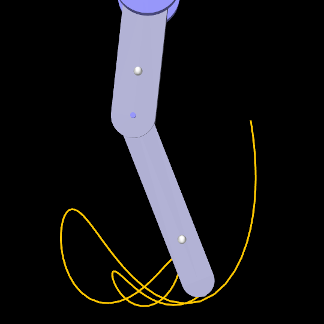
\includegraphics[width=2.5in]{images/LineTracing}
 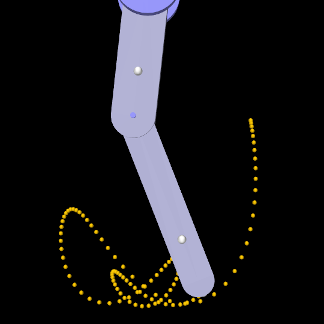
\includegraphics[width=2.5in]{images/PointTracing}
\fi
\end{tabular}
\end{center}
\caption{Left: tracing applied to the distal marker of
{\tt MultiJointedArm}. Right: same trace, with
{\sf pointTracing} enabled.}
\label{PointLineTracing:fig}
\end{figure}

\begin{sideblock}
Tracing probes can also be created and edited interactively,
as described in the section ``Point Tracing'' of the
\artisynthManual{uiguide}{ArtiSynth User Interface Guide}.
\end{sideblock}

\subsection{Position probes}
\label{PositionProbes:sec}

Applications often find it useful to parametrically control the position of
point or frame-based components, which include
\javaclass[\mech]{Point},
\javaclass[\mech]{Frame},
\javaclass[\mech]{FixedMeshBody}.
and their subclasses
(e.g., \javaclass[\mech]{Particle},
\javaclass[\mech]{RigidBody},
and
\javaclass[\fem]{FemNode3d}).
This can be done by setting either the components' {\sf position} or {\sf
targetPosition} properties, and (for frame-based components) their {\sf
orientation} or {\sf targetOrientation} properties. As described
in Section \ref{targetPositions:sec}, setting {\sf
targetPosition} and {\sf targetOrientation} is often preferable as this will
automatically update the component's velocity, and so provide more information
to the integrator, whereas setting {\sf position} and {\sf orientation} will
leave the velocity unchanged.

\begin{sideblock}
When controlling the position and/or velocity of dynamic components, which
include {\tt Point} and {\tt Frame}, it is important to ensure that their {\sf
dynamic} property is set to {\tt false} and that they are
unattached. Otherwise, the dynamic simulation will override any attempt at
setting their position or velocity.
\end{sideblock}

For frame-based components, the {\sf orientation} and {\sf targetOrientation}
properties describe their spatial orientation using an instance of
\javaclass[maspack.matrix]{AxisAngle}, which represents
a single rotation $\theta$ about a specific axis $\u$ in world coordinates (any
3D rotation can be expressed this way). However, when using this in a probe to
control or observe a frame-based component's pose over time, a couple
of issues arise:

\begin{itemize}

\item There are other rotation representations that may be more
useful or easier to specify, such as z-y-x or x-y-z rotations,
in either radians or degrees.

\item Whatever rotation representation is used, care must be taken
when interpolating it between knot points. Rotations cannot be treated as
vectors and interpolation must instead take the form of curves on the 3D
rotation group $SO(3)$. The details are beyond the scope of this document but
were initially described by Shoemake \cite{shoemake1985animating}.

\end{itemize}

To address these issues, ArtiSynth supplies
\javaclass[\probes]{PositionInputProbe} and
\javaclass[\probes]{PositionOutputProbe}, which can be used to control or
observe the position of one or more points or frame-based components, while
offering a variety of rotation representations and handling rotation
interpolation correctly. In particular, {\tt PositionInputProbe}s
allow an application to supply key-frame animation control poses for
frame-based components.

{\tt PositionInputProbe}s can be created with the constructors
%
\begin{methodtable}{0.9}{0.1}
\midline
%
\methodentry
{\probes.PositionInputProbe.PositionInputProbe(String,ModelComponent,,,double)}%
{PositionInputProbe (String name, ModelComponent comp, RotationRep rotRep,\brh
boolean useTargetProps, double startTime, double stopTime)}%
{\ }%
%
\methodspace{0.5em}%
\methodentry
{\probes.PositionInputProbe.PositionInputProbe(String,Collection,,,,double)}%
{PositionInputProbe (String name, Collection<? extends ModelComponent> comps,\brh
RotationRep rotRep, 
boolean useTargetProps, double startTime, double stopTime)}%
{\ }%
%
\methodspace{0.5em}%
\methodentry
{\probes.PositionInputProbe.PositionInputProbe(String,ModelComponent,,,String)}%
{PositionInputProbe (String name, ModelComponent comp, RotationRep rotRep,\brh
boolean useTargetProps, String filePath)}%
{\ }%
%
\methodspace{0.5em}%
\methodentry
{\probes.PositionInputProbe.PositionInputProbe(String,Collection,,,String)}%
{PositionInputProbe (String name, Collection<? extends ModelComponent> comps,\brh
RotationRep rotRep, boolean useTargetProps, String filePath)}%
{\ }%
%%
%\methodspace{0.5em}%
%\brh
\midline
\end{methodtable}
%
In the above, {\tt name} is the probe name (optional, can be {\tt null}), and
{\tt comp} and {\tt comps} refer to the component(s) to be assigned to the
probe; as indicated above, these must be instances of {\tt Point}, {\tt Frame},
or {\tt FixedMeshBody}. {\tt rotRep} is an instance of 
\javaclass[maspack.matrix]{RotationRep}, which indicates 
how rotations should be represented, as described further below.  The argument
{\tt useTargetProps}, if {\tt true}, specifies that the probe should be
attached to the {\sf targetPosition} and (for frames) {\sf targetOrientation}
properties, vs. the {\sf position} and {\sf orientation} properties (if {\tt
false}). {\tt startTime} and {\tt stopTime} give the probe's start and stop
times, while {\tt filePath} specifies a probe file from which to read in the
probe's basic parameters and data, per Section \ref{DataFileFormat:sec}.  Probes
constructed without a file need to have data added, as per Section
\ref{probeDataInCode:sec}.

As indicated by the constructors, {\tt NumericInputProbe}s can control multiple
point and frame-based components, and this arrangement affects the size and
composition of the data vector. Each point component requires 3 numbers
specifying position, while each frame components requires $3 + r$ numbers
specifying position and orientation, where $r$ is the size of the of the
rotation representation. Although the {\tt orientation} and {\tt
targetOrientation} properties describe rotation using an
\javaclass[maspack.matrix]{AxisAngle}, this will be converted
into knot point data based on the assigned {\tt RotationRep}, with $r$ equal to
either 3 or 4. The total $m$ of the data vector is then
%
\begin{equation*}
m = 3 n_p + (3 + r) n_f
\end{equation*}
%
where $n_p$ is the number of points and $n_f$ is the number of frames.

\javaclass[maspack.matrix]{RotationRep} provides a variety of ways
to specify the rotation and applications can choose the most suitable:

\begin{description}

\item[ZYX]\mbox{}

Successive rotations, in radians, about the $z-y-x$ axes; $r = 3$.

\item[ZYX\_DEG]\mbox{}

Successive rotations, in degrees, about the $z-y-x$ axes; $r = 3$.

\item[XYZ]\mbox{}

Successive rotations, in radians, about the $x-y-z$ axes; $r = 3$.

\item[XYZ\_DEG]\mbox{}

Successive rotations, in degrees, about the $x-y-z$ axes; $r = 3$.

\item[AXIS\_ANGLE]\mbox{}

Axis-angle representation ($u$, $\theta$), with the $\theta$ given in
radians; $r = 4$. The axis $u$ does not need to be normalized.

\item[AXIS\_ANGLE\_DEG]\mbox{}

Axis-angle representation ($u$, $\theta$), with the $\theta$ given in
degrees; $r = 4$. The axis $u$ does not need to be normalized.

\item[QUATERNION]\mbox{}

Unit quaternion; $r = 4$.

\end{description}

As a possibly more convenient alternative to the methods of
Section \ref{probeDataInCode:sec}, and to avoid having to explicitly pack the
position and orientation information into the probe's knot data, {\tt
PositionInputProbe}s also supply the following methods to set the knot data for
individual components being controlled by the probe:

%
\begin{methodtable}{0.7}{0.3}
\midline
%
\methodentry
{\probes.PositionInputProbe.setPointData()}%
{setPointData (Point point, double time, Vector3d pos)}%
{Set point position at a given time.}%
%
\methodentry
{\probes.PositionInputProbe.setPointData()}%
{setPointData (ModelComponent frame, double time,\brh RigidTransform3d TFW)}%
{Set frame position/orientation at a given time.}%
%
%\methodspace{0.5em}%
%\brh
\midline
\end{methodtable}
%
Each of these methods writes only the portion of the knot point at the
indicated time that corresponds to the specified component; other portions are
left unchanged or initialized to 0. For frames, {\tt TFW} gives the pose
(position/orientation) in the form of the transform from frame to world
coordinates, and the orientation is transformed into knot point data according
the the probe's rotation representation.

\javaclass[\probes]{PositionOutputProbe}s can be created
with constructors analogous to {\tt PositionInputProbe}:
%
\begin{methodtable}{0.9}{0.1}
\midline
%
\methodentry
{\probes.PositionOutputProbe.PositionOutputProbe(,ModelComponent,,,double)}%
{PositionOutputProbe (String name, ModelComponent comp, RotationRep rotRep,\brh
double startTime, double stopTime)}%
{\ }%
%
\methodspace{0.5em}%
\methodentry
{\probes.PositionOutputProbe.PositionOutputProbe(,Collection,,,double)}%
{PositionOutputProbe (String name, Collection<? extends ModelComponent> comps,\brh
RotationRep rotRep, 
double startTime, double stopTime)}%
{\ }%
%
\methodspace{0.5em}%
\methodentry
{\probes.PositionOutputProbe.PositionOutputProbe(,ModelComponent,,,,,)}%
{PositionOutputProbe (String name, ModelComponent comp, RotationRep rotRep,\brh
String filePath, double startTime, double stopTime, double interval)}%
{\ }%
%
\methodspace{0.5em}%
\methodentry
{\probes.PositionOutputProbe.PositionOutputProbe(,Collection,,,,,)}%
{PositionOutputProbe (String name, Collection<? extends ModelComponent> comps,\brh
RotationRep rotRep, String filePath, double startTime, double stopTime, 
double interval)}%
{\ }%
%%
%\methodspace{0.5em}%
%\brh
\midline
\end{methodtable}
%
The knot data format is the same as for {\tt PositionInputProbe}s, with
rotations represented according to the setting of {\tt rotRep}.  There is no
{\tt useTargetProps} argument because {\tt PositionOutputProbe}s bind only to
the {\sf position} and {\sf orientation} properties. If present, the {\tt
filePath} and {\tt interval} arguments specify an attached file name for saving
probe data and the update interval in seconds. Setting {\tt interval} to -1
causes updating to occur at the simulation update rate, and this is the default
for constructors without an {\tt interval} argument.


\subsection{Velocity probes}

As with positions, applications may sometimes need to parametrically control or
observe the velocity of point or frame-based components, which include
\javaclass[\mech]{Point}, \javaclass[\mech]{Frame},
and their subclasses (but not {\tt FixedMeshBody}, as this is not a dynamic
component and so does not maintain a velocity).  This can be done by setting
either the components' {\sf velocity} or {\sf targetVelocity} properties, with
the latter sometimes preferable as it will automatically update the component's
position, whereas setting {\sf velocity} will not. For frame-based components,
{\sf velocity} and {\sf targetVelocity} are described by a
6-DOF \javaclass[maspack.spatialmotion]{Twist} component that contains both
translational and angular velocities. Unlike with finite rotations, there is
only one representation for angular velocity (as a vector with units of
radians/sec) and there are no interpolation issues.

When the position of a component is being controlled it is typically not
necessary to also supply velocity information. This is especially true for
position probes bound to {\sf targetPosition} and {\sf targetOrientation}
properties, since these update velocity information automatically. However, for
position probes bound to {\sf position} and {\sf orientation}, it can be
sometimes be useful to use a velocity probe to also supply velocities.  One
example of this is when components are being tracked by inverse simulation
(Chapter
\cite{InverseSimulation:sec}), as this extra information this can reduce
tracking error and lag.

ArtiSynth provides 
\javaclass[\probes]{VelocityInputProbe} and
\javaclass[\probes]{VelocityOutputProbe}
to controller or monitor the velocities of one or more point or frame-based
components. The constructors for these are:
%
\begin{methodtable}{0.9}{0.1}
\midline
%
\methodentry
{\probes.VelocityInputProbe.VelocityInputProbe(String,ModelComponent,,double)}%
{VelocityInputProbe (String name, ModelComponent comp, 
boolean useTargetProps,\brh double startTime, double stopTime)}%
{\ }%
%
\methodspace{0.5em}%
\methodentry
{\probes.VelocityInputProbe.VelocityInputProbe(String,Collection,,,double)}%
{VelocityInputProbe (String name, Collection<? extends ModelComponent> comps,\brh
boolean useTargetProps, double startTime, double stopTime)}%
{\ }%
%
\methodspace{0.5em}%
\methodentry
{\probes.VelocityInputProbe.VelocityInputProbe(String,ModelComponent,,String)}%
{VelocityInputProbe (String name, ModelComponent comp,
boolean useTargetProps,\brh String filePath)}%
{\ }%
%
\methodspace{0.5em}%
\methodentry
{\probes.VelocityInputProbe.VelocityInputProbe(String,Collection,,String)}%
{VelocityInputProbe (String name, Collection<? extends ModelComponent> comps,\brh
boolean useTargetProps, String filePath)}%
{\ }%
\methodspace{1.05em}%
%%
\methodentry
{\probes.VelocityOutputProbe.VelocityOutputProbe(,ModelComponent,,double)}%
{VelocityOutputProbe (String name, ModelComponent comp,\brh
double startTime, double stopTime)}%
{\ }%
%
\methodspace{0.5em}%
\methodentry
{\probes.VelocityOutputProbe.VelocityOutputProbe(,Collection,,double)}%
{VelocityOutputProbe (String name, Collection<? extends ModelComponent> comps,\brh
double startTime, double stopTime)}%
{\ }%
%
\methodspace{0.5em}%
\methodentry
{\probes.VelocityOutputProbe.VelocityOutputProbe(,ModelComponent,,,,)}%
{VelocityOutputProbe (String name, ModelComponent comp,
String filePath,\brh double startTime, double stopTime, double interval)}%
{\ }%
%
\methodspace{0.5em}%
\methodentry
{\probes.VelocityOutputProbe.VelocityOutputProbe(,Collection,,,,)}%
{VelocityOutputProbe (String name, Collection<? extends ModelComponent> comps,\brh
String filePath, double startTime, double stopTime, 
double interval)}%
{\ }%
%\methodspace{0.5em}%
%\brh
\midline
\end{methodtable}
%
For all of these, the arguments are completely analogous to those for the
constructors of {\tt PositionInputProbe} and {\tt PositionOutputProbe}, with
the argument {\tt rotRep} absent because it is not needed, and with {\tt
useTargetProps} specifying whether the probe should be attached to the {\sf
targetVelocity} or {\tt velocity} properties.

If a position probe (either input or output) exists for a given collection of
components, it is possible to automatically create a {\tt VelocityInputProbe}
for the same set of components, using one of the following static methods:
%
\begin{methodtable}{0.65}{0.35}
\midline
%
\methodentry
{\probes.VelocityInputProbe.createNumeric()}%
{VelocityInputProbe VelocityInputProbe.createNumeric (String name,\brh 
NumericProbeBase source, double interval)}%
{Create by numeric differentiation.}%
%
\methodspace{0.5em}%
\methodentry
{\probes.VelocityInputProbe.createInterpolated()}%
{VelocityInputProbe VelocityInputProbe.createInterpolated (String name,\brh 
NumericProbeBase source, double interval)}%
{Create by interpolation.}%
%
\midline
\end{methodtable}
%
Both take an optional probe {\tt name} and {\tt source} probe. The update {\tt
interval} gives the time interval between the created knot points, with -1
causing this to be taken from the source. The first method creates the probe by
numeric differentiation of the source's position data and should be used only
when the source's data is dense, while the second method finds the derivative
from the {\it interpolation method} of the source probe (as described by {\tt
getInterpolationOrder()}) and is better suited when the source data is sparse
(although the resulting velocity will not be continuous unless the
interpolation order is greater than linear).

The following code fragments creates a position probe and then uses this to
generate a velocity probe:
%
\begin{lstlisting}[]
   PositionInputProbe posProbe;
   VelocityInputProbe velProve;
   String bodyFilePath;
   RigidBody body; 
   ...
   boolean useTargetProps = true;
   posProbe = new PositionInputProbe (
      "body position", body, RotationRep.XYZ, useTargetProps, bodyFilePath);
   velProbe = VelocityInputProbe.createNumeric (
      "body velocity", posProbe, /*interval*/-1);
\end{lstlisting}
%

\subsection{Example: controlling a point and frame}

\begin{figure}[ht]
\begin{center}
\begin{tabular}{cc}
\iflatexml
  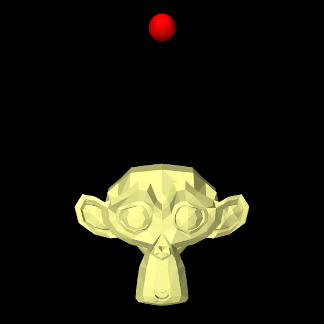
\includegraphics[]{images/PositionProbes0}&
  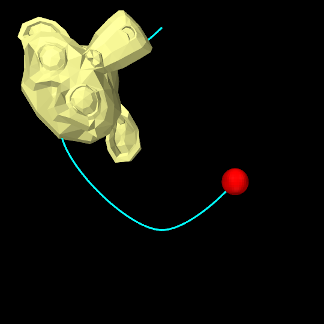
\includegraphics[]{images/PositionProbes1}\\
\else
  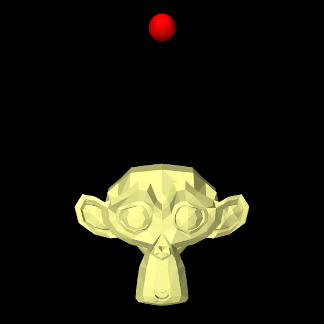
\includegraphics[height=2.5in]{images/PositionProbes0}&
  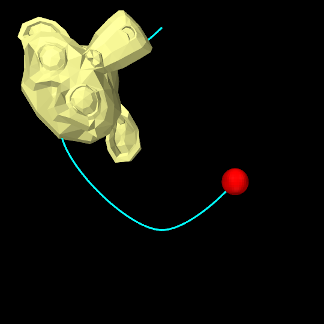
\includegraphics[height=2.5in]{images/PositionProbes1}\\
\fi
\end{tabular}
\end{center}
\caption{Left: {\tt PositionProbes} when first loaded. Right: model running,
showing the point and monkey orbiting around each other and the particle
trace in cyan.}
\label{PositionProbes:fig}
\end{figure}

A model demonstrating position and velocity probes is defined in
%
\begin{verbatim}
  artisynth.demos.tutorial.PositionProbes
\end{verbatim}
%
It creates a point and a rigid body (using the Blender monkey mesh), sets both
to be non-dynamic, uses position and velocity probes to control their
positions, and uses {\tt PositionOutputProbe} and {\tt VelocityOutputProbe} to
monitor the resulting positions and velocities. The model class definition,
excluding the include directives, is shown here:
%
\lstset{numbers=left}
\iflatexml
%% Hack: latexml lstinputlisting doesn't handle firstline correctly
\lstset{firstnumber={-26}}
\lstinputlisting[firstline=1]{../../src/artisynth/demos/tutorial/PositionProbes.java}
\lstset{firstnumber={1}}
\else
\lstinputlisting[firstline=28]{../../src/artisynth/demos/tutorial/PositionProbes.java}
\fi
\lstset{numbers=none}
%
The {\tt build()} creates a {\tt MechModel} and then adds to it a rigid body
(created from the Blender monkey mesh) and a particle (lines 8-19).  Both
components are made non-dynamic to allow their positions and velocities to be
controlled, and references to them are placed a list used to create the probes
(lines 21-24).

A {\tt PositionInputProbe} for controlling the positions is created at lines
26-44, using a rotation representation of {\tt RotationRep.ZYX} (successive
rotations about the z-y-x axes, in radians). For this example, the {\tt
useTargetProps} is set to {\tt false} (so that the probe binds to {\sf
position} and {\sf orientation}), because we are going to be specifying
velocities explicitly using another probe. Data for the probe is set using {\tt
setData()}, with the point and monkey positions/poses specified, in order, for
times 0, 0.5, 1.0, 1.5 and 2. As per the rotation specification, poses for the
monkey are given by 3 positions and 3 z-y-x rotations. Because the data is
sparse, the probe's interpolation order is set to {\tt Cubic} to generate
smooth motions.

A {\tt VelocityInputProbe} is created by differentiated the position probe
(lines 47-49); {\tt createInterpolated()} is used because the position data is
sparse and so numeric differentiation would yield bad results.

Finally, output probes to track both the resulting positions and velocities,
together with a tracing probe to render the point's path in cyan, are created
at lines 51-65. When creating the {\tt PositionOutputProbe}, we use the same
rotation representation {\tt RotationRep.ZYX} as for the input probe, but this
is not necessary. For example, if one were to instead specify {\tt
RotationRep.QUATERNION}, then the frame orientations would be specified as
quaternions.

To run this example in ArtiSynth, select {\sf All demos > tutorial >
PositionProbes} from the {\sf Models} menu. When run, both the point and monkey
will orbit around each other, with the point path being displayed by the tracing
probe (Figure \ref{PositionProbes:fig}, right).

\begin{figure}[ht]
\begin{center}
\begin{tabular}{cc}
\iflatexml
  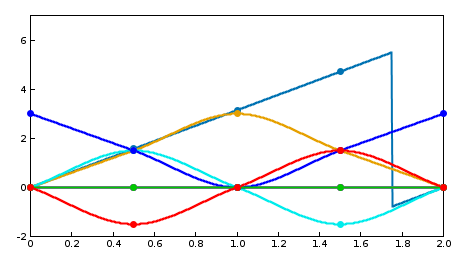
\includegraphics[]{images/PositionInputProbeData}&
  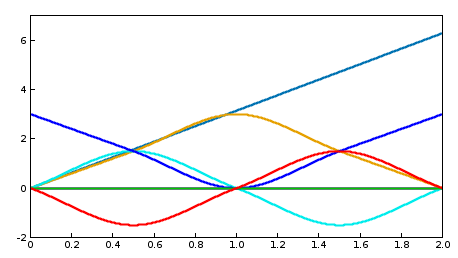
\includegraphics[]{images/PositionOutputProbeData}\\
\else
  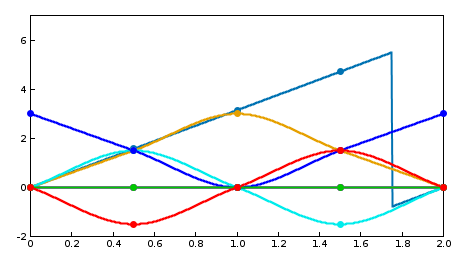
\includegraphics[width=3.25in]{images/PositionInputProbeData}&
  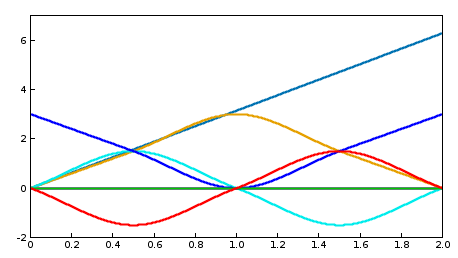
\includegraphics[width=3.25in]{images/PositionOutputProbeData}\\
\fi
\end{tabular}
\end{center}
\caption{Left: plot of the {\tt PositionInputProbe} data,
showing a discontinuity at $t = 1.75$ for monkey's $y$ axis rotation data.
Right: plot of the {\tt PositionOutputProbe} data shows the continuity
of the actual trajectory.}
\label{PositionIOProbes:fig}
\end{figure}

Several things about this demo should be noted:

\begin{itemize}

\item The use of {\tt setData()} in creating the position probe could 
be replaced by
\javamethod[\probes.PositionInputProbe]{setPointData()} and
\javamethod[\probes.PositionInputProbe]{setFrameData()}, as per
%
\begin{lstlisting}[]
  pip.setPointData (point, 0.5, new Point3d(-1.5,0,1.5)); 
  pip.setPointData (point, 1.0, new Point3d(0,0,0)); 
  pip.setPointData (point, 1.5, new Point3d(1.5,0,1.5));

  pip.setFrameData (monkey, 0.5, new RigidTransform3d(1.5,0,1.5, 0,PI/2,0));
  pip.setFrameData (monkey, 1.0, new RigidTransform3d(0.0,0,3.0, 0,PI,0));
  pip.setFrameData (monkey, 1.5, new RigidTransform3d(-1.5,0,1.5, 0,3*PI/2,0));
\end{lstlisting}
%
Here, we can omit data for times 0 and 2 (at the probe's start and end) because
the motion begins and ends at the components' initial positions, for which data
was automatically added when the probe was created. (Likewise, data for times 0
and 2 could be omitted in the original code if {\tt addData()} was used instead
of {\tt setData()}).

\item Position probes handle angle wrapping correctly.
In the position input probe, the y-axis rotation for the monkey goes
from $3 \pi/2$ to $0$ between $t = 1.5$ and $t = 2$.  However, by generating
``minimal distance'' motions, interpolation proceeds as though the final angle
was specified as $2 \pi$, allowing the circular motion to complete instead of
backtracking (although in the display plot, there is an apparent discontinuity
at $t = 1.75$; see Figure \ref{PositionIOProbes:fig}, left).  Likewise, in
position output probes, as data is added, the rotation representation is
chosen to be as near as possible to the previous, so that in the
example the recorded $y$ rotation does indeed arrive at $2 \pi$ instead of $0$
(Figure \ref{PositionIOProbes:fig}, right).

\item Since {\tt useTargetProps} is set to {\tt false} in the example,
the velocity input probe is needed to set the component velocities; if this
probe is made inactive (either in code or interactively in the timeline), then
while the bodies will still move, no velocities will be set and the data in the
velocity output probe will be uniformly 0.

Alternatively, if {\tt useTargetProps} is set to {\tt true}, then the input
probes will be bound to {\sf targetPosition}, {\sf targetOrientation}, and {\sf
targetVelocity}, and both positions and velocities will be set for the
components if {\it either} input probe is active. Reflecting the description in
Section \ref{targetPositions:sec}:

\begin{itemize}

\item If the position input probe is {\it active} and the velocity input probe
is {\it inactive}, then the velocities will be determined by {\it
differentiating} the target position inputs (albeit with a one-step time lag).

\item If the position input probe is {\it inactive} and the velocity input probe
is {\it active}, then the positions will be determined by {\it integrating} the
target velocity inputs. Note that in this case, when the probes terminate, the
components will continue moving with their last specified velocity.

\item If {\it both} the position and velocity input probes are active,
then both the target position and velocity information will be used to update
the component positions and velocities.
	
\end{itemize}

This provides a useful example of how target properties work.

\end{itemize}

\subsection{Numeric monitor probes}
\label{NumericMonitorProbes:sec}

In some cases, it may be useful for an application to deploy an output probe in
which the data, instead of being collected from various component properties,
is generated by a function within the probe itself. This ability is provided by
a
\javaclass[\probes]{NumericMonitorProbe}, which generates
data using its  \javamethodAlt{%
\probes.NumericMonitorProbe.generateData()}%
{generateData(vec,t,trel)}
method. This evaluates a vector-valued function of time at
either the absolute time {\tt t} or the probe-relative time {\tt trel}
and stores the result in the vector {\tt vec}, whose size equals the
vector size of the probe (as returned by
\javamethod[\probes.NumericProbeBase]{getVsize()}).  The
probe-relative time {\tt trel} is determined by
%
\begin{equation}
\text{trel} = (\text{t} - \text{tstart})/\text{scale}
\end{equation}
%
where {\tt tstart} and {\tt scale} are the probe's start time
and scale factors as returned by
\javamethod[\probes.Probe]{getStartTime()} and
\javamethod[\probes.Probe]{getScale()}.

As described further below, applications have several ways to control
how a {\tt NumericMonitorProbe} creates data:

\begin{itemize}

\item Provide the probe with a
\javaclass[\probes]{DataFunction} using the
\javamethodAlt{\probes.NumericDataFunctionProbe.setDataFunction()}%
{setDataFunction(func)} method;

\item Override the \javamethodAlt{%
\probes.NumericMonitorProbe.generateData()}%
{generateData(vec,t,trel)}
method;

\item Override the \javamethodAlt{%
\probes.NumericMonitorProbe.apply(double)}{apply(t)}
method.

\end{itemize}

The application is free to generate data in any desired way, and so in
this sense a {\tt NumericMonitorProbe} can be used similarly to a {\tt
Monitor}, with one of the main differences being that the data
generated by a {\tt NumericMonitorProbe} can be automatically displayed
in the ArtiSynth GUI or written to a file.

The \javaclass[\probes]{DataFunction} interface
declares an {\tt eval()} method,
%
\begin{verbatim}
   void eval (VectorNd vec, double t, double trel)
\end{verbatim}
%
that for 
{\tt NumericMonitorProbe}s
evaluates a vector-valued function of time,
where the arguments take the same role as for the monitor's \javamethodAlt{%
\probes.NumericMonitorProbe.generateData()}%
{generateData()}
method. Applications can declare an appropriate {\tt DataFunction} and
set or query it within the probe using the methods
% method table
\begin{lstlisting}[]
   void setDataFunction (DataFunction func);

   DataFunction getDataFunction();
\end{lstlisting}
%
The default implementation {\tt generateData()} checks to see
if a data function has been specified, and if so, uses that to
generate the probe data. Otherwise, if the probe's data function is {\tt
null}, the data is simply set to zero.

To create a {\tt NumericMonitorProbe} using a supplied {\tt DataFunction},
an application will create a generic probe instance, using one
of its constructors such as 
%
\begin{lstlisting}[]
   NumericMonitorProbe (vsize, filePath, startTime, stopTime, interval);
\end{lstlisting}
%
and then define and instantiate a {\tt DataFunction} and pass it to
the probe using {\tt setDataFunction()}. It is not necessary to supply
a file name (i.e., {\tt filePath} can be {\tt null}), but if one is
provided, then the probe's data can be saved to that file.

A complete example
of this is defined in
%
\begin{verbatim}
  artisynth.demos.tutorial.SinCosMonitorProbe
\end{verbatim}
%
the listing for which is:

\lstset{numbers=left}
\lstinputlisting{../../src/artisynth/demos/tutorial/SinCosMonitorProbe.java}
\lstset{numbers=none}

In this example, the {\tt DataFunction} is implemented using the class
{\tt SinCosFunction}, which also implements
\javaclass[maspack.util]{Clonable} and the associated {\tt clone()}
method. This means that the resulting probe will also be duplicatable
within the GUI. Alternatively, one could implement {\tt
SinCosFunction} by extending
\javaclass[\probes]{DataFunctionBase}, which implements
{\tt Clonable} by default. Probes containing {\tt DataFunction}s
which are {\it not} {\tt Clonable} will not be duplicatable.

When the example is run, the resulting probe output is shown in the
timeline image of Figure \ref{sinCosProbe:fig}.

\begin{figure}[ht]
\begin{center}
\iflatexml
 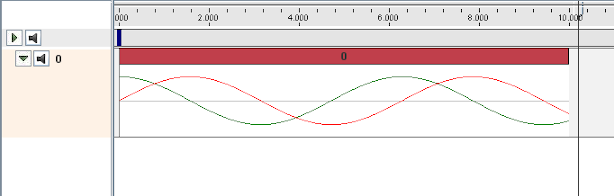
\includegraphics[]{images/sinCosProbe}
\else
 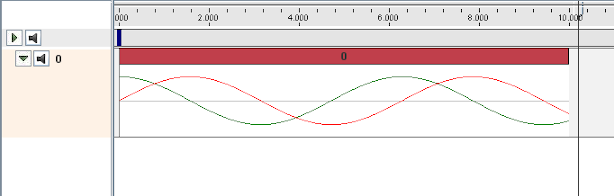
\includegraphics[width=4.5in]{images/sinCosProbe}
\fi
\end{center}
\caption{Output from a {\tt NumericMonitorProbe} which generates sine
and cosine waves.}
\label{sinCosProbe:fig}
\end{figure}

As an alternative to supplying a {\tt DataFunction} to a generic {\tt
NumericMonitorProbe}, an application can instead subclass {\tt
NumericMonitorProbe} and override either its \javamethodAlt{%
\probes.NumericMonitorProbe.generateData()}%
{generateData(vec,t,trel)} or \javamethodAlt{%
\probes.NumericMonitorProbe.apply(double)}{apply(t)}
methods. As an example of the former, one could create a subclass as
follows:
%
\begin{lstlisting}[]
  class SinCosProbe extends NumericMonitorProbe {
     
     public SinCosProbe (
        String filePath, double startTime, double stopTime, double interval) {
        super (2, filePath, startTime, stopTime, interval);
     }

     public void generateData (VectorNd vec, double t, double trel) {
        vec.set (0, Math.sin (t));
        vec.set (1, Math.cos (t));        
     }
  }
\end{lstlisting}
%
Note that when subclassing, one must also create constructor(s) for
that subclass. Also, {\tt NumericMonitorProbe}s which don't have a
{\tt DataFunction} set are considered to be clonable by default, which
means that the {\tt clone()} method may also need to be overridden if
cloning requires any special handling.

\subsection{Numeric control probes}
\label{NumericControlProbes:sec}

In other cases, it may be useful for an application to deploy an input
probe which takes numeric data, and instead of using it to modify
various component properties, instead calls an internal method to
directly modify the simulation in any way desired.  This ability is
provided by a \javaclass[\probes]{NumericControlProbe},
which applies its numeric data using its \javamethodAlt{%
\probes.NumericControlProbe.applyData()}%
{applyData(vec,t,trel)} method. This receives the numeric input data
via the vector {\tt vec} and uses it to modify the simulation for
either the absolute time {\tt t} or probe-relative time {\tt
trel}. The size of {\tt vec} equals the vector size of the probe (as
returned by
\javamethod[\probes.NumericProbeBase]{getVsize()}), and
the probe-relative time {\tt trel} is determined as described in
Section \ref{NumericMonitorProbes:sec}.

A {\tt NumericControlProbe} is the {\tt Controller} equivalent
of a {\tt NumericMonitorProbe}, as described in Section 
\ref{NumericMonitorProbes:sec}. Applications have several ways to control
how they apply their data:

\begin{itemize}

\item Provide the probe with a 
\javaclass[\probes]{DataFunction} using the
\javamethodAlt{\probes.NumericDataFunctionProbe.setDataFunction()}%
{setDataFunction(func)} method;

\item Override the \javamethodAlt{%
\probes.NumericControlProbe.applyData()}%
{applyData(vec,t,trel)}
method;

\item Override the \javamethodAlt{%
\probes.NumericControlProbe.apply(double)}{apply(t)}
method.

\end{itemize}

The application is free to apply data in any desired way, and so in
this sense a {\tt NumericControlProbe} can be used similarly to a
{\tt Controller}, with one of the main differences being that the
numeric data used can be automatically displayed in the ArtiSynth GUI
or read from a file.

The \javaclass[\probes]{DataFunction} interface
declares an {\tt eval()} method,
%
\begin{verbatim}
   void eval (VectorNd vec, double t, double trel)
\end{verbatim}
%
that for 
{\tt NumericControlProbe}s applies the numeric data, 
where the arguments take the same role as for the monitor's \javamethodAlt{%
\probes.NumericControlProbe.applyData()}%
{applyData()}
method. Applications can declare an appropriate {\tt DataFunction} and
set or query it within the probe using the methods
% method table
\begin{lstlisting}[]
   void setDataFunction (DataFunction func);

   DataFunction getDataFunction();
\end{lstlisting}
%
The default implementation {\tt applyData()} checks to see
if a data function has been specified, and if so, uses that to
apply the probe data. Otherwise, if the probe's data function is {\tt
null}, the data is simply ignored and the probe does nothing.

To create a {\tt NumericControlProbe} using a supplied {\tt DataFunction},
an application will create a generic probe instance, using one
of its constructors such as 
% method table
\begin{lstlisting}[]
   NumericControlProbe (vsize, data, startTime, stopTime, timeStep);

   NumericControlProbe (filePath);
\end{lstlisting}
%
and then define and instantiate a {\tt DataFunction} and pass it to
the probe using {\tt setDataFunction()}. The latter constructor
creates the probe and reads in both the data and timing information
from the specified file.

\begin{figure}[ht]
\begin{center}
\iflatexml
 \includegraphics[]{images/spinControlProbe}
\else
 \includegraphics[width=4.5in]{images/spinControlProbe}
\fi
\end{center}
\caption{Screen shot of the {\tt SpinControlDemo}, showing the
numeric data in the timeline.}
\label{spinControlProbe:fig}
\end{figure}

A complete example
of this is defined in
%
\begin{verbatim}
  artisynth.demos.tutorial.SpinControlProbe
\end{verbatim}
%
the listing for which is:

\lstset{numbers=left}
\lstinputlisting{../../src/artisynth/demos/tutorial/SpinControlProbe.java}
\lstset{numbers=none}

This example creates a simple box and then uses a {\tt
NumericControlProbe} to spin it about the $z$ axis, using a {\tt
DataFunction} implementation called {\tt SpinFunction}. A clone method
is also implemented to ensure that the probe will be duplicatable in
the GUI, as described in Section \ref{NumericMonitorProbes:sec}.  A
single channel of data is used to control the orientation angle of the
box about $z$, as shown in Figure \ref{spinControlProbe:fig}.

Alternatively, an application can subclass {\tt NumericControlProbe}
and override either its \javamethodAlt{%
\probes.NumericControlProbe.applyData()}%
{applyData(vec,t,trel)} or \javamethodAlt{%
\probes.NumericControlProbe.apply(double)}{apply(t)}
methods, as described for {\tt NumericMonitorProbe}s (Section
\ref{NumericMonitorProbes:sec}).

\section{Working with TRC data}

The TRC data format was originally developed by Motion Analysis Corporation to
describe marker position data acquired during motion capture. An overview of
the format is provided as part of the
\href{https://opensimconfluence.atlassian.net/wiki/spaces/OpenSim/pages/53089972/Marker+.trc+Files}{OpenSim
documentation}.

ArtiSynth supplies a simple reader and writer for TRC data, with the reader
able to create probes directly from TRC files and the writer able to write
files directly from probes.

\begin{sideblock}
It is assumed the TRC data is tab delimited; files that do not use tabs to
separate their data will not be readable. There may also be other limitations of
which we are unaware.
\end{sideblock}

\subsection{TRC reader}
\label{TRCReader:sec}

\javaclass[\probes]{TRCReader} allows one to read TRC data from a file using
the simple code fragment
%
\begin{lstlisting}[]
import artisynth.core.probes.TRCReader;
...

  File trcFile;
  ...
  TRCReader reader = new TRCReader (trcFile);
  reader.readData();
\end{lstlisting}
%
A constructor also exists that accepts a string file name argument.

\begin{sideblock}
Both the constructors and the {\tt readData()} method throw an {\tt
IOException}, which must either be handled in a {\tt try/catch} block or thrown
by the calling method.
\end{sideblock}

Once the data has been read, it may be queried with the following methods:
%
\begin{methodtable}{0.5}{0.5}
\midline
%
\methodentry
{\probes.TRCReader.numFrames()}%
{int numFrames()}%
{Return the number of frames.}%
%
\methodentry
{\probes.TRCReader.getFrameTime()}%
{double getFrameTime (int fidx)}%
{Return time of the fidx-th frame.}%
%
\methodentry
{\probes.TRCReader.numMarkers()}%
{int numMarkers()}%
{Return the number of markers.}%
%
\methodentry
{\probes.TRCReader.getMarkerLabels()}%
{ArrayList<String> getMarkerLabels()}%
{Return all the marker labels.}%
%
\methodentry
{\probes.TRCReader.getMarkerIndex()}%
{int getMarkerIndex (String label)}%
{Return index of the labeled marker.}%
%
\methodentry
{\probes.TRCReader.getMarkerPositions(int)}%
{ArrayList<Point3d> getMarkerPositions (int fidx)}%
{Return all marker positions at frame fidx.}%
%
\methodentry
{\probes.TRCReader.getMarkerPositions(VectorNd,int)}%
{void getMarkerPositions (VectorNd mpos, int fidx)}%
{Return all marker positions at frame fidx into mpos.}%
%
\methodentry
{\probes.TRCReader.getMarkerPosition(int,int)}%
{Point3d getMarkerPosition (int fidx, int midx)}%
{Return position of midx-th marker at frame fidx.}%
%
\methodentry
{\probes.TRCReader.getMarkerPosition(int,String)}%
{Point3d getMarkerPosition (int fidx, String label)}%
{Return position of labeled marker at frame fidx.}%
%
%\methodspace{0.5em}%
%\brh
\midline
\end{methodtable}
%
Both the frame and marker indices in the above methods are 0-based.

{\tt TRCReader} also supplies the following methods for
creating {\tt PositionInputProbe}s directly from the data:
%
\begin{methodtable}{0.9}{0.1}
%\midline
%
\methodentry
{\probes.TRCReader.createInputProbe(,,,,)}%
{PositionInputProbe createInputProbe (String name, 
Collection<? extends Point> points,\brh
boolean useTargetProps, double startTime, double stopTime)}%
{\ }%
\methodspace{0.5em}%
%
\methodentry
{\probes.TRCReader.createInputProbeUsingLabels(,,,,)}%
{PositionInputProbe createInputProbeUsingLabels (String name, 
Collection<? extends Point> points,\brh
List<String> labels, boolean useTargetProps, double startTime, double stopTime)}%
{\ }%
%
%\midline
\end{methodtable}
%
For these, {\tt name} is the probe name (optional, can be {\tt null}), {\tt
points} are the points to which the probe should be attached, {\tt
useTargetProps} indicates if the {\sf targetPosition} or {\sf position}
properties should be bound, {\tt startTime} and {\tt stopTime} give the
start and stop times, and {\tt labels}, if present, gives a list of the marker
labels that should be used for each point; otherwise, points are assigned to
marker data in order.

As a convenience, the following static methods are also supplied:

\begin{methodtable}{0.9}{0.1}
%\midline
%
\methodentry
{\probes.TRCReader.createInputProbe(,,,)}%
{PositionInputProbe createInputProbe (String name, 
Collection<? extends Point> points,\brh
File trcFile, boolean useTargetProps)}%
{\ }%
%
\methodspace{0.5em}%
%
\methodentry
{\probes.TRCReader.createInputProbeUsingLabels(,,,,)}%
{PositionInputProbe createInputProbeUsingLabels (String name, 
Collection<? extends Point> points,\brh
List<String> labels, File trcFile, boolean useTargetProps)}%
{\ }%
%
%\midline
\end{methodtable}
%
These read the data directly from the supplied TRC file, assigning the probe a
start time of 0 and a stop time determined from the last frame time.

\subsection{TRC writer}
\label{TRCWriter:sec}

\javaclass[\probes]{TRCWriter} allows an application to write a TRC file
directly from the data in a numeric probe, using a code fragment such as
%
\begin{lstlisting}[]
import artisynth.core.probes.TRCWriter;
...

  File trcFile;
  NumericProbeBase probe;

  ...
  TRCWriter writer = new TRCWriter (trcFile);
  reader.writeData (probe, /*labels*/null);
\end{lstlisting}
%
A constructor also exists that accepts a string file name argument.

The full signature for {\tt writeData()} is
%
\begin{methodtable}{0.7}{0.3}
%
\methodentry
{\probes.TRCWriter.writeData()}%
{void writeData (NumericProbeBase probe, List<String> labels)}%
{\ }%
%
\end{methodtable}
%
where {\tt probe} is any type of probe associated with {\sf position} or {\sf
targetPosition} properties for a set of \javaclass[\mech]{Point} components.
The {\tt labels} argument is an optional list of marker labels that should be
assigned to the data for each point. If this is not supplied, labels are
assigned automatically, either from the point names, or when these are null, by
prepending {\tt "mkr"} to the marker index.

\begin{sideblock}
The {\tt writeData()} method throws an {\tt IOException}, which must either be
handled in a {\tt try/catch} block or thrown by the calling method.
\end{sideblock}

{\tt TRCWriter} also supplies a few methods that can be used
to format the data before it is written:
%
\begin{methodtable}{0.5}{0.5}
\midline
%
\methodentry
{\probes.TRCWriter.getNumberFormat()}%
{String getNumberFormat()}%
{Return the format string for float data.}%
%
\methodentry
{\probes.TRCWriter.setNumberFormat()}%
{void setNumberFormat (String fmtStr)}%
{Set the format string for float data.}%
%
\methodentry
{\probes.TRCWriter.getUnitsString()}%
{String getUnitsString()}%
{Return the string used to represent units.}%
%
\methodentry
{\probes.TRCWriter.setUnitsString()}%
{void setUnitsString (String str)}%
{Set the string used to represent units.}%
%
\midline
\end{methodtable}
%

For convenience, the following static methods are also provided:
%
\begin{methodtable}{0.7}{0.3}
%
\methodentry
{\probes.TRCWriter.write(File,,)}%
{void write (File file, NumericProbeBase probe, List<String> labels)}%
{\ }%
\methodspace{0.5em}%
%
\methodentry
{\probes.TRCWriter.write(String,,)}%
{void write (String fileName, NumericProbeBase probe, List<String> labels)}%
{\ }%
%
\end{methodtable}

\subsection{Example: moving MultiJointedArm with TRC data}
\label{TRCMultiJointedArm:sec}

\begin{figure}[t]
\begin{center}
\iflatexml
 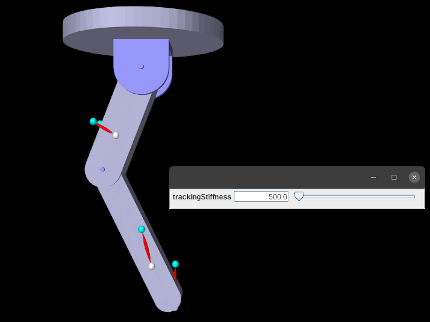
\includegraphics[]{images/TRCMultiJointedArm}
\else
 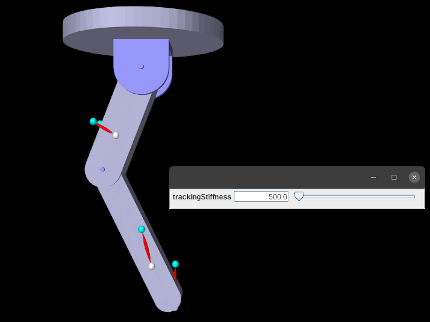
\includegraphics[width=4in]{images/TRCMultiJointedArm}
\fi
\end{center}
\caption{{\tt TRCMultiJointedArm}, overlaid with the tracking stiffness
control panel. The tracking stiffness itself is set low enough that
the springs (red) between the target points (cyan) and markers (white)
are visible.}
\label{TRCMultiJointedArm:fig}
\end{figure}

The example model
%
\begin{verbatim}
  artisynth.demos.tutorial.TRCMultiJointedArm
\end{verbatim}
%
illustrates several features that have been introduced in this chapter.  It
extends the model {\tt MultiJointedArm}, previously described in
Section \ref{MultiJointedArm:sec}. Then it reads TRC data defining target
trajectories for the markers attached to the arm, with the intention of moving
the arm. While a standard way to make marker data move an articulated structure
is to employ an inverse kinematic solver (Section \ref{XXX}), this example
uses a simpler solution. For each marker, a target point is defined and
attached to it by means of a spring. The target points (which are non-dynamic)
are then moved by means of a {\tt PositionInputProbe} created from the TRC
data. As they move, they drag the markers (and the attached bodies) around by
means of the resulting spring forces. It can be shown that the resulting rest
position of the system is identical to that of the inverse kinematic solver of
Section \ref{XXX} (assuming equal marker weights).

Tracking accuracy increases with spring stiffness (although very high
stiffnesses may cause stability issues). To illustrate this relationship, a
control panel is created that allows the user to adjust the spring stiffness
interactively. To be able to control the stiffness of one spring with a single
parameter, a custom model property, called {\sf trackingStiffness}, is created
per the description of Section \ref{CustomProperties:sec}, to control the
stiffness values for all the springs.

The model's class definition, excluding include directives, is given in
%
\lstset{numbers=left}
\iflatexml
%% Hack: latexml lstinputlisting doesn't handle firstline correctly
\lstset{firstnumber={-21}}
\lstinputlisting[firstline=1]{../../src/artisynth/demos/tutorial/TRCMultiJointedArm.java}
\lstset{firstnumber={1}}
\else
\lstinputlisting[firstline=23]{../../src/artisynth/demos/tutorial/TRCMultiJointedArm.java}
\fi
\lstset{numbers=none}
%
The first parts of the code define the {\sf trackingStiffness} property, by
first creating a local static property list ({\tt myProps}) that inherits from
the parent class {\tt MultiJointedArm.class} (lines 9-10). A static block adds
the property definition (lines 12-16), and the new list is made visible by a
local implementation of {\tt getAllPropertyInfo()} (lines 18-20).  Get/set
accessors are then defined for the property (lines 22-36). The property value
is kept in the member variable {\tt myTrackingStiffness}, but when it is set
the stiffness is updated for all springs stored in the {\tt MechModel}'s axial
spring list.

The {\tt build()} method starts by calling {\tt super.build()} to create the
original {\tt MultiJointedArm} model (line 39), after which a reference to the
created {\tt MechModel} will be stored in the inherited member {\tt myMech}.
Then for each model marker, a target point is created, together with a
connecting axial spring (lines 41-50). For simplicity, the targets and springs
are stored in the {\tt MechModel}'s default {\tt points} and {\tt axialSprings}
lists, but they could be stored in custom containers, as per
Section \ref{GeneralComponentArrangements:sec}.

Next, TRC marker data is read from the file {\tt "data/multiJointMkrs.trc"}
located relative to the model's source folder, using the {\tt TRCReader}
described in Section \ref{TRCReader:sec}. This is used to create a {\tt
PositionInputProbe} attached to the target points (which are located under {\tt
myMech.points()}) (lines 57-60). Lastly, a control panel is created to allow
adjustment of the tracking stiffness, and some render properties are set.

The last part of the class definition overrides the method {\tt
postscanInitialize()}, which is called in place of the {\tt build()} method
when a model is read from an ArtiSynth {\tt .art} file. This method should
initialize any class members which are unknown to the component hierarchy and
would normally be set in the {\tt build()} method.  In this case, it is
necessary to initialize {\tt myMech}, which is needed by {\tt
setTrackingStiffness()} and would otherwise not be set.  Models which are not
intended to be saved to {\tt .art} files do not need to override {\tt
postscanInitialize()}.

To run this example in ArtiSynth, select {\sf All demos > tutorial >
TRCMultiJointedArm} from the {\sf Models} menu. The demo will appear, together
with the control panel (shown overlaid in Figure
\ref{TRCMultiJointedArm:fig}). When the model is run, the target points will be
moved under the control of their position probe, dragging the markers along via
the attached springs. Increasing/decreasing the spring stiffness will
decrease/increase the tracking error.

\section{Application-Defined Menu Items}
\label{MenuItems:sec}

Application models can define custom {\it menu items} that appear
under the {\tt Application} menu in the main ArtiSynth menu bar.

This can be done by implementing the interface
\javaclass[artisynth.core.modelbase]{HasMenuItems} in either the {\tt
RootModel} or any of its top-level components (e.g., models,
controllers, probes, etc.). The interface contains a single
method
% method table
\begin{lstlisting}[]
   public boolean getMenuItems(List<Object> items);
\end{lstlisting}
%
which, if the component has menu items to add, should append them
to {\tt items} and return {\tt true}.

The {\tt RootModel} and all models derived from
\javaclass[artisynth.core.modelbase]{ModelBase} implement {\tt
HasMenuItems} by default, but with {\tt getMenuItems()} returning {\tt
false}. Models wishing to add menu items should override this default
declaration. Other component types, such as controllers, need to
explicitly implement {\tt HasMenuItems}.

\begin{sideblock}
Note: the {\sf Application} menu will only appear if {\tt getMenuItems()} returns
{\tt true} for either the {\tt RootModel} or one or more of its
top-level components.
\end{sideblock}

\javamethod*[artisynth.core.modelbase.HasMenuItems]{getMenuItems()}
will be called each time the {\sf Application} menu is selected, so the
menu itself is created on demand and can be varied to suite the
current system state. In general, it should return items that are
capable of being displayed inside a Swing {\tt JMenu}; other items
will be ignored. The most typical item is a Swing {\tt JMenuItem}.  The
convenience method
\javamethodAlt{maspack.widgets.GuiUtils.createMenuItem()}%
{createMenuItem(listener,text,toolTip)}
can be used to quickly create menu items, as in the following
code segment:
%
\begin{lstlisting}[]
   public boolean getMenuItems(List<Object> items) {
      items.add (GuiUtils.createMenuItem (this, "reset", ""));
      items.add (GuiUtils.createMenuItem (this, "add sphere", ""));
      items.add (GuiUtils.createMenuItem (this, "show flow", ""));
      return true;
   }
\end{lstlisting}
%
This creates three menu items, each with {\tt this} specified as an
{\tt ActionListener} and no tool-tip text, and appends them
to {\tt items}. They will then appear under the {\sf Application}
menu as shown in Figure \ref{applicationMenu:fig}.

\begin{figure}[t]
\begin{center}
\iflatexml
 \includegraphics[]{images/applicationMenu}
\else
 \includegraphics[width=2.5in]{images/applicationMenu}
\fi
\end{center}
\caption{Application-defined menu items appearing under the ArtiSynth
menu bar.}
\label{applicationMenu:fig}
\end{figure}

To actually execute the menu commands, the items returned by {\tt
getMenuItems()} need to be associated with an {\tt ActionListener}
(defined in {\tt java.awt.event}), which supplies the method {\tt
actionPerformed()} which is called when the menu item is
selected. Typically the {\tt ActionListener} is the component
implementing {\tt HasMenuItems}, as was assumed in the example
declaration of {\tt getMenuItems()} shown above. {\tt RootModel} and
other models derived from {\tt ModelBase} implement {\tt ActionListener} by
default, with an empty declaration of {\tt actionPerformed()} that
should be overridden as required.
A declaration of {\tt actionPerformed()} capable of handling the menu
example above might look like this:
%
\begin{lstlisting}[]
   public void actionPerformed (ActionEvent event) {
      String cmd = event.getActionCommand();
      if (cmd.equals ("reset")) {
         resetModel();
      }
      else if (cmd.equals ("add sphere")) {
         addSphere();
      }
      else if (cmd.equals ("show flow")) {
         showFlow();
      }
   }
\end{lstlisting}
%

\subsection{Smoothing probe data}
\label{SmoothingProbeData:sec}

Numeric probe data can also be smoothed, which is convenient for removing noise
from either input or output data. Different smoothing methods are available; at
the time of this writing, they include:

\begin{description}

\item[Moving average] \mbox{}

Applies a mean average filter across the knots, using a moving window
whose size is specified by the {\sf window size} field. The window is
centered on each knot, and is reduced in size near the end knots to
ensure a symmetric fit. The end knot values are not changed.  The
window size must be odd and the {\sf window size} field enforces this.

\item[Savitzky Golay] \mbox{}

Applies Savitzky-Golay smoothing across the knots, using a moving
window of size $w$.  Savitzky-Golay smoothing works by fitting the
data values in the window to a polynomial of a specified degree $d$, and
using this to recompute the value in the middle of the window.  The
polynomial is also used to interpolate the first and last $w/2$
values, since it is not possible to center the window on these.

The window size $w$ and the polynomial degree $d$ are specified by the
{\sf window size} and {\sf polynomial degree} fields. $w$ must be odd,
and must also be larger than $d$, and the fields enforce these
constraints.

\end{description}

These operations may be applied with the following numeric probe
methods:

%
\begin{methodtable}{0.5}{0.5}
\midline
%
\methodentry
{\probes.NumericProbeBase.smoothWithMovingAverage()}%
{void smoothWithMovingAverage (double winSize)}%
{Moving average smoothing over a specified window.}%
%
\methodentry
{\probes.NumericProbeBase.smoothWithSavitzkyGolay()}%
{void smoothWithSavitzkyGolay (\brh double winSize, int deg)}%
{Savitzky Golay smoothing with specified window and degree.}%
%
\midline
\end{methodtable}
%

%
\ifdefined\maindoc
\else
\end{document}
\fi

XXX talk about target positions
